\documentclass{article}
\usepackage{graphicx} % Required for inserting images
\usepackage{hyperref}
\usepackage[top=1.2in, bottom=1.2in, left=3cm, right=3cm, a4paper]{geometry}
\usepackage{subcaption}
\usepackage{ragged2e}
\usepackage{amsmath}
\begin{document}

\thispagestyle{empty}
\begin{center}
    	\begin{figure} [t]
		
\includegraphics[width=0.2\linewidth]{../fig/logo_UGA.png}
		\hspace{8.0cm}
		
\includegraphics[width=0.2\linewidth]{../fig/logo_IGE.png}
		\vspace{2.0cm}
	    \end{figure}

        \begin{Large}
        \textbf{Numerical experiments in glacial inceptions in Northern Europe} 
        \end{Large}
        
        \vspace{0.8cm}
        \textbf{ESPELETA BOLIVAR, Ruben Dario}\\
        \vspace{3.0cm}
        \textbf{Research project}\\
	    Presented in partial fulfillment of the requirements for the degree of\\
	    \textbf{Master applied mechanics}\\
        \vspace{3.0cm}

        Université Grenoble Alpes\\
        \textbf{\today}
        \vspace{4.0cm}
\end{center}
\flushleft{
    Project advisor(s):\\
    Ph.D. Cruz García Molina
}
\clearpage

\begin{center}
	\textbf{\Large{Abstract}}
\end{center}

\vspace{0.5cm}

\justifying

The present project aims to develop a numerical experiment to understand the impact of important parameters in the glacier dynamics, such as the grounding line. Using the finite element method Elmer/Ice, simulations on idealized topographies are proposed, which are set up in the context of the CalvingMIP inter-comparison project, that aims to develop different models to simulate and to improve calving laws in ice sheet models. Using these idealized topographies, the numerical experiments are performed using resolutions varying from 10km until 1km, starting from an initial state where there is no ice, until the formation of the glacier. The objective of the study is to evaluate the impact of the resolution on the prediction of the grounding line position after the system has reached the steady state. The analysis of the results are contrasted with the theory and show the convergence of the behaviour of the grounding line position for higher resolutions, where the differences start to be lower.

\vspace{3cm}

\clearpage
\tableofcontents

\pagebreak

\section{Introduction}
\justifying
Ice sheets are important components of global climate systems \cite{zhang2017comparison}. The impacts of the perturbation of these climate systems are most acutely changes in global sea level, as ice sheets grow or decay in response to climate forcing and internally controlled dynamics. While the rate of present-day sea-level rise is dominated by ocean steric changes and eustatic changes due to shrinking mountain glaciers, the eustatic contribution from the large ice sheets (Greenland and Antarctic) has increased in recent decades and it is expected to continue increasing in coming decades and centuries \cite{clark2015recent}. To have a better idea, if all the ice were to melt completely, the sea level would rise by an estimated 65m \cite{morlighem2017bedmachine, haywood2011pliocene} and force populations to emigrate their land submerged by water.

In order to understand these impacts on the dynamics and melting of ice sheets and glaciers, numerical models are developed. Through these models, some of them which are based on finite elements, we can have simulations that can make better predictions of future ice sheets' behavior and rate of sea level rise, and ultimately provide policymakers with improved estimates of future change.

\begin{figure}[!h]
	\centering
	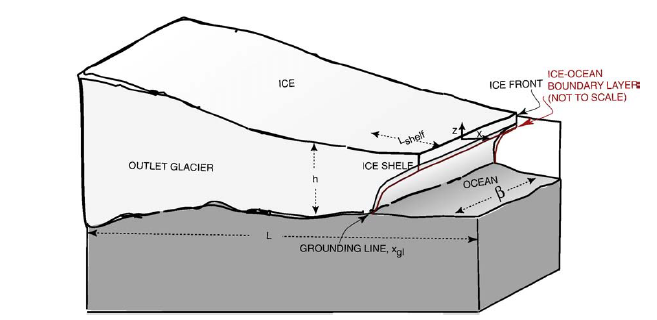
\includegraphics[width=0.7\linewidth]{../fig/Scheme_grounding_line.png}
	\caption{Schematic simplified diagram of the model domain of a glacier \cite{parizek2010implications}}
	\label{groundingline}
\end{figure}

There are different variables that play an important role in the dynamics of the glaciers. There is, for example, the grounding line. Its location is still a topic of discussion in the literature surrounding ice sheet dynamics \cite{goldberg2018representing}.

\begin{figure}[!h]
	\centering
	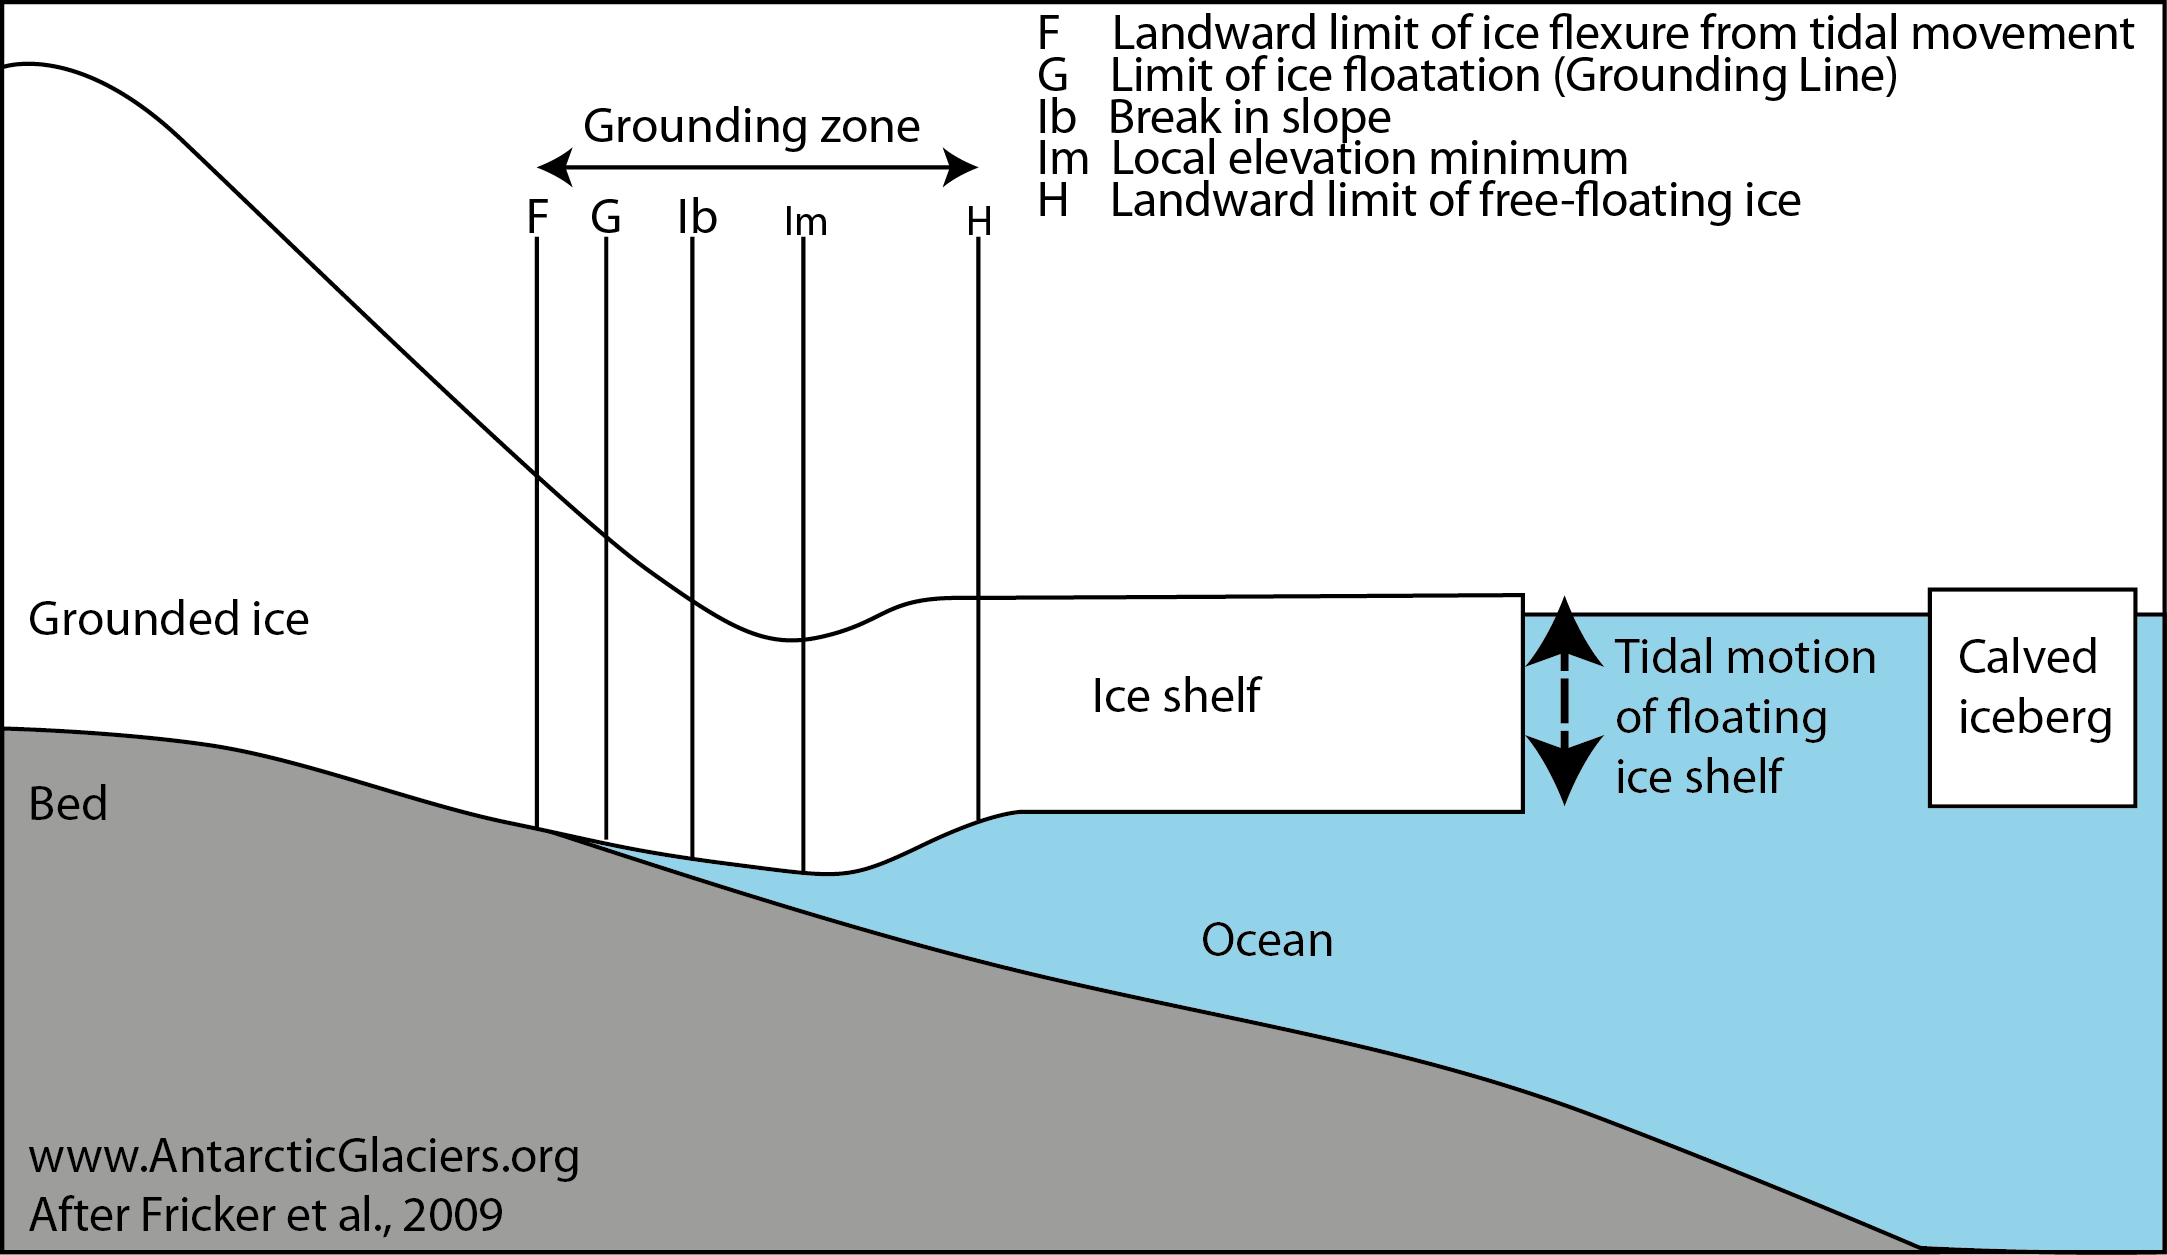
\includegraphics[width=0.7\linewidth]{../fig/groundingzone.png}
	\caption{Schematic of a tributary glacier where we can observe the different parts denoting the grounding zone \cite{fricker2009mapping}.}
	\label{groundingzone}
\end{figure}

Glaciers that end in the ocean are called tidewater glaciers. Glaciers that flow into an ice shelf are called tributary glaciers as the one shown in figure \ref{groundingline} by \cite{parizek2010implications}. The line that divides the part of the glacier that is in contact with the solid bedrock and the ice shelf floating on water driven by buoyancy, is called the grounding line \cite{cheng2019full}. The location of the grounding line is important because the mass loss from glaciers is strongly linked to changes in the ice shelves and their grounding lines \cite{brunt2010mapping,pritchard2012antarctic}. Its long-term horizontal position is very susceptible to temporal and spatial changes in ice thickness and sea level, as well as bedrock and ice surface slopes. Ice thinning and rising sea levels can cause grounding lines to retreat while thickening or declining sea levels can cause an advance \cite{friedl2020remote}. It is important to know the grounding line position to be able to quantify the ice discharge into the sea and as an indicator, if the ice sheet is advancing or retreating \cite{konrad2018net}.

Grounding lines are actually more of a zone. The grounding zone is the region where ice transitions from a grounded ice sheet to a freely floating ice shelf, typically over several kilometers. The grounding zone is the region between point F in figure \ref{groundingzone} by \cite{fricker2009mapping}, where there is no tidal movement, and point H, which is the seaward limit of ice flexure, where the ice is free-floating. The floating ice shelf changes in elevation in response to tides, atmospheric air, pressure, and oceanic processes. Grounding occurs when the ice shelf comes into contact with the bedrock below \cite{fricker2009mapping}. The transition from grounded ice sheets to floating ice shelves plays an important role in controlling marine ice sheet dynamics, as it determines the rate at which ice flows out of the grounded part of the ice sheet \cite{schoof2007ice}. This is because ice flux through the grounding line increases sharply with ice thickness at the grounding line. This means that grounding lines are unstable on reverse-bed slopes, such as those under Pine island glaciers, because recession into deeper water increases ice flux and further encourages more glacier recession \cite{schoof2007marine}.

 This project aims to understand the direct impact of changes in the position of the grounding line on the flow dynamics of ice sheets glaciers. We will use the finite element model Elmer/Ice to explore the spatial resolution impact on the grounding line position. We will compare the changes in the position of the grounding line for two different idealized topographies. This will let us understand the behavior of real present and past glaciers such as the Northern European glacier. 

 \section{Glacier dynamics}
 \subsection{Mass and movement balance equations}
 An ice sheet is a continuous sheet of land ice that covers a very large area of several thousand to millions of square meters. It is formed by an accumulation of snow which will densify under its own weight until it becomes ice. This ice will then flow downhill under its weight, and can eventually reach the sea. If it does, and the ice propagates above the sea, this part of the ice sheet is called an ice shelf \cite{hutter1982mathematical}. Figure \ref{groundingline} shows a diagram of an ice sheet showing different parts of it, such as the ice shelf, and some phenomena happening inside of it, such as the ice flow or the snow accumulation.

 For large time scales the ice is considered a very viscous fluid. The ice flow equations are then derived from the Stokes equation \cite{hutter1982mathematical}:
\begin{equation}
	div\sigma + \rho g = div\tau - gradp + \rho g = 0;
\end{equation}
with $\sigma$ the stress tensor, $\rho$ the density of the ice, g the gravity vector, $\tau$ the deviatoric stress tensor, with $\sigma = \tau - pI$ and $p=\frac{tr\sigma}{3}$. 

And the mass conservation:
\begin{equation}
	\frac{dh}{dt}+ div(uH)=M_s + M_b;
\end{equation}
With $u$ the velocity, H the ice thickness, $M_s$ and $M_b$ the mass balance at the surface and at the bottom respectively. $M_s$ will be defined, and $M_b$ is considered as 0 for convenience purposes. 

The stresses are related to the viscosity and the strain by Glen's law \cite{glen1958flow}:
\begin{equation}
	\tau = 2\eta\dot{\epsilon},
\end{equation}
with the viscosity given by:
\begin{equation}
	\eta = \frac{1}{2}(EA)^\frac{-1}{n} \dot{\epsilon_e}^\frac{(1-n)}{n}.
\end{equation}
Where:
\begin{itemize}
	\item The strain rate $\dot{\epsilon}$.
	\item Glen's constant n=3.
	\item The enhancement factor to account for an anisotropic effect E=1.
	\item The rheological parameter A=15,46.
\end{itemize}
For an ice sheet, the ratio of the vertical length over the horizontal length is more than $1:10^3$. Indeed, the thickness of an ice sheet goes from 0 m to a few thousand of meters (e.g. the ice sheet in Greenland is 3300 m thick at most \cite[]{bamber2001new}) and the typical horizontal length of an ice sheet is of the order of magnitude of 1000 km. This allows us to apply the shallow ice approximation. It assumes a large ratio of horizontal to vertical length, that the basal shear stress is balanced by  the gravitational driving stress, and a large vertical to horizontal stress ratio. That represents a slow flow in the interior of an ice sheet (blue regions in Figure \ref{velocityglaciar}). The approximation makes the method computationally cheaper than the Full-Stokes model with good accuracy over long simulations.

\begin{figure}[!h]
	\centering
	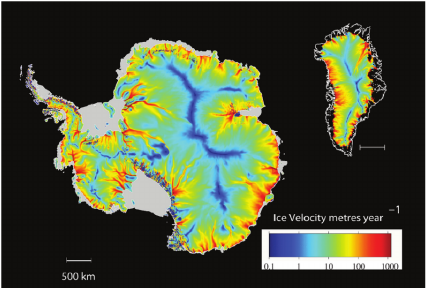
\includegraphics[width=0.7\linewidth]{../fig/velocityglaciar.png}
	\caption{Ice velocities in Antarctica and Greenland topographies, where we can see in red the highest velocity profiles in the glaciers and as a consequence we consider the basal shear stress as 0 and the longitudinal stress dominates, which allows using a Shallow Shelf approximation \cite[]{allison2009ice}.}
	\label{velocityglaciar}
\end{figure}
Figure \ref{velocityglaciar} shows a map of velocities in Antarctica and Greenland topographies. Where this velocity is the highest, the basal shear stress cannot be considered balanced by gravity anymore. Instead, it is taken as 0 and the longitudinal stress dominates. This is the Shallow Shelf approximation, initially developed for ice shelves, but which has been extended to dragging ice streams. It is a 2D vertically integrated model, the ice velocity being depth-averaged.

But these approximations are not mandatory: the Full Stokes model is still the most precise, it accounts for all nine stress components. It is useful around the parts that are at the limits of the other models or over complex topographies, but not needed for the interior of ice sheets, where the improvement would be minimal but the computational cost way higher \cite{larour2012continental}.

The factors such as sensitivity, long time intervals, and long distances require careful treatment of the groundline neighborhood by the numerical method to discretize the model equations \cite{cheng2019full}. The most accurate ice model is the Full Stokes (FS) equations \cite{cheng2019full}. However, a simplification of these FS equations by integrating into the depth of the ice is the shallow shelf approximation \cite{macayeal1989large}. The computational advantage with Shallow Shelf approximation is that the dimension of the problem is reduced by one, it is often used for simulations of the interaction between a grounded ice sheet and a marine ice shelf \cite{cheng2019full}. 
In this project, only the Shallow Shelf approximation is made, as this is how future projections of Greenland and Antarctica are done with the Elmer/Ice model.

\subsection{Grounding line stability}

A long debate on the dynamics of such ice sheets was initiated in the 1970s when \cite{weertman1974stability} proposed that a marine ice sheet that lies on an upward-sloping bed is unstable. Recently, the instability hypothesis has been strongly reinforced, based on a boundary-layer theory due to \cite{schoof2007ice}. Moreover, \cite{vieli2005assessing} showed the poor ability of marine ice-sheet models to give consistent prognostic results and, more particularly, they highlighted the influence of the grid size on model results. One of their main conclusions was that no reliable model was able to predict grounding line dynamics at the time of their study.

There is a need to improve marine ice-sheets models in order to corroborate recent theoretical predictions and to obtain confident simulations of the grounding line dynamics. \cite{durand2009marine} proposed a full-Stokes solution of the ice-sheet/ice-shelf transition. This approach has been built on literature dealing with the coupling between a grounded ice sheet and a floating ice shelf and identifying this transition zone as a crucial control of the marine ice sheet dynamics \cite[]{weertman1974stability, van1985response, chugunov1996modelling, hindmarsh1996stability, vieli2005assessing, schoof2007ice, schoof2007marine}.

\cite{durand2009full} showed, using the finite element code Elmer/Ice, that the full-Stokes modeling of the ice-sheet/ice-shelf transition gives a consistent prediction of grounding-line migration. However, their approach is highly sensitive to the chosen mesh resolution. For a grid size smaller than $5 km$ in the grounding-line vicinity, predictions start to be consistent. For any finer resolution than $5 km$, the steady-state grounding-line position is the same (6km is the standard deviation). If a sub-grid refinement of 200m in the vicinity of the grounding line is applied the steady-state position is stable.

In order to study and test the behavior of the different components of the models, idealized systems are studied and, based on the results that are obtained from these idealized cases, the hypothesis, models, and numerical methods used to solve the problems are improved. For this reason, within the framework of this project, we will analyze the behavior of the Elmer/Ice method to solve idealized systems and topographies. The framework in which the present project is focused is on the study of the Northern Europe glacier. But, since this glacier does not exist anymore, idealized cases simulations of North Europe glaciers, such as Greenland can be analyzed as mentioned before, and their results can be used to improve the numerical models, hypothesis, and parameters of the models, and this way we can better understand the behavior of ancient glaciers such as the Northern Europe glacier.

 \section{Numerical model}
 \subsection{The Elmer/Ice finite element method}
 Most of the time analytical solutions are challenging or even impossible to obtain. In order to model ice sheets, both the finite difference method (FDM) and the finite element method (FEM) are used. The finite difference method consists in converting ordinary and partial differential equations into a system of linear equations by approximating derivatives as finite differences. Elmer/Ice, on the other hand, uses the finite element method.
 The ice sheet/ice flow model Elmer/Ice includes developments related to glaciological problems and a large number of dedicated solvers and user functions that solve the Full-Stokes equations for various ice rheologies (classical, Glenn's flow law, anisotropic laws, and porous compressible firns/snow law). It includes solvers for the classical asymptotical expansions of the Stokes equations, namely the shallow ice approximation and the shallow and shallow shelf approximation (SSA). All these equations can be solved diagnostically or transiently, allowing the displacement of the boundaries.

 Elmer/Ice considers a continuum as an assembly of non-overlapping elements forming the same geometry, which makes the modeling of complex geometries possible. Each element is made of at least two points, which are applied to the forces and computed the displacements. To solve the equations, Elmer/Ice uses subroutines or solvers. Each equation corresponds to one solver to be referenced in the input file, together with the different parameters of the problem. They each compute the evolution of given variables, such as the ice thickness or the velocity, to give at each time step a picture of the flow. All combined, it allows us to visualize the evolution of the flow through time.

 Here I can put the figures showing the mesh for a quarter domain for thule and the cone.

\subsection{Tophographic profiles}
This numerical experiment uses two different topographic profiles. A cone and a more realistic topography (Thule).
\subsubsection{Cone}
	The idealized model consists of a circular bedrock configuration (Figure \ref{circular_topo_top}) given by:
	\begin{equation}
		\theta=arctan2(y,x);
	\end{equation}
	\begin{equation}
		I=R-cos(2\theta)\frac{R}{2}
	\end{equation}
	\begin{equation}
		Bed_0=Bc-(Bc-BI)\frac{|x^2+y^2|}{R2}^;
	\end{equation}
	Where $R=800x10^3 m$, $Bc=0.9 x 10^3 m$, and $BI=-2 x 10^3 m$. 
	\begin{figure}[!h]
		\centering
		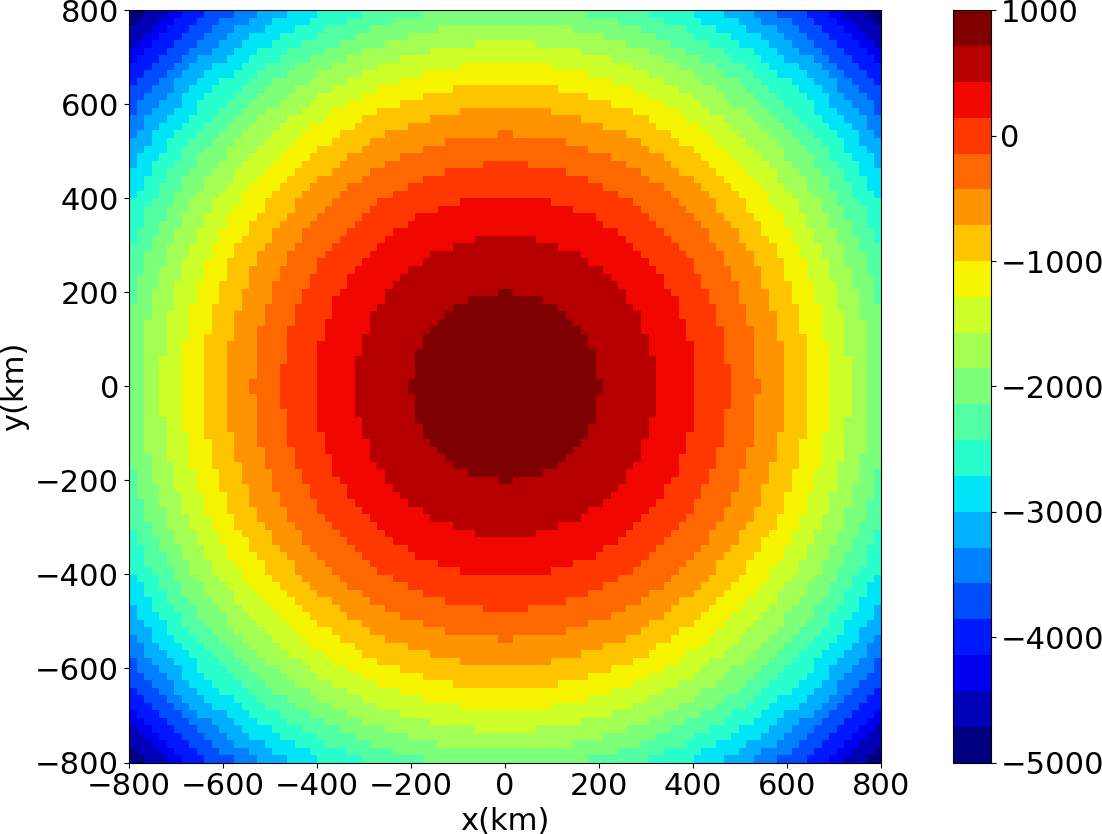
\includegraphics[width=0.45\linewidth]{../fig/circular_topo_top.png}
		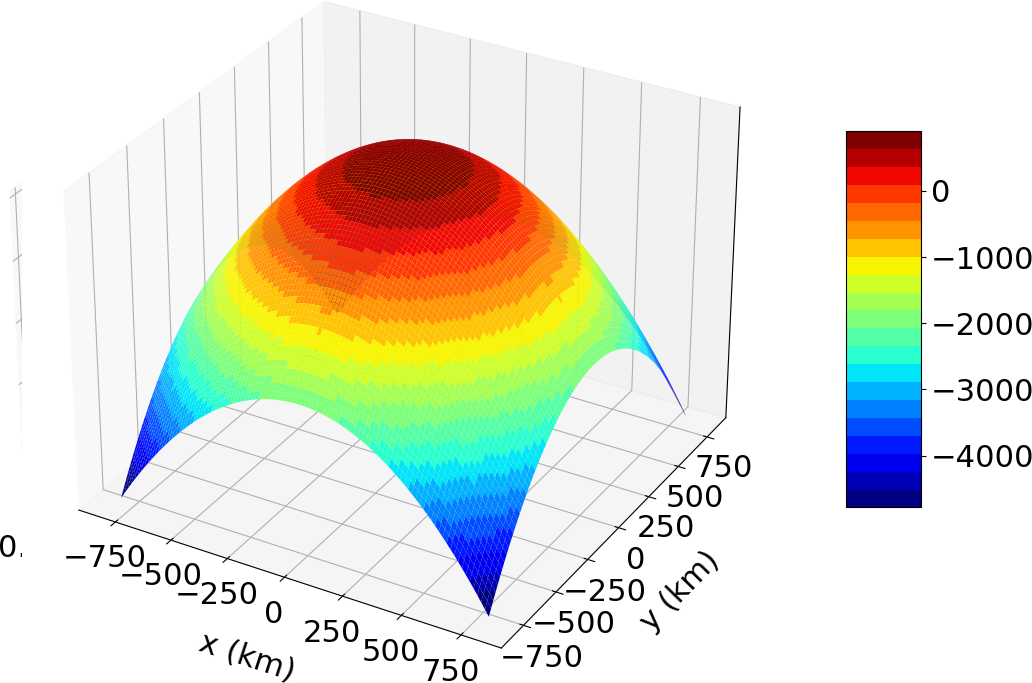
\includegraphics[width=0.45\linewidth]{../fig/circular_topo_jet}
		\caption{Circular bedrock topography. On the left side top view and on the right side, lateral view.}
		\label{circular_topo_top}
	\end{figure}
 
 \subsubsection{Thule}
 The Thule bedrock configuration is shown in Figure \ref{Thule_3D} and \ref{Thule_3D1} and is given by:
	\begin{equation}
		\theta=arctan2(y,x);
	\end{equation}
	\begin{equation}
		I=R-cos(2\theta)\frac{R}{2};
	\end{equation}
	\begin{equation}
		Bed_0=Bc-(Bc-BI)\frac{|x^2+y^2}{R^2};
	\end{equation}
	\begin{equation}
		Bed=Bacos(3\pi\frac{\sqrt[2]{x^2+y^2}}{I})+Bed_0;
	\end{equation}
	With $R=800 x 10^3 m$, $Bc=0,9 x 10^3 m$, $BI=-2 x 10^3 m$, and $Ba=1,1 x 10^3$.
	\begin{figure}[!h]
		\centering
		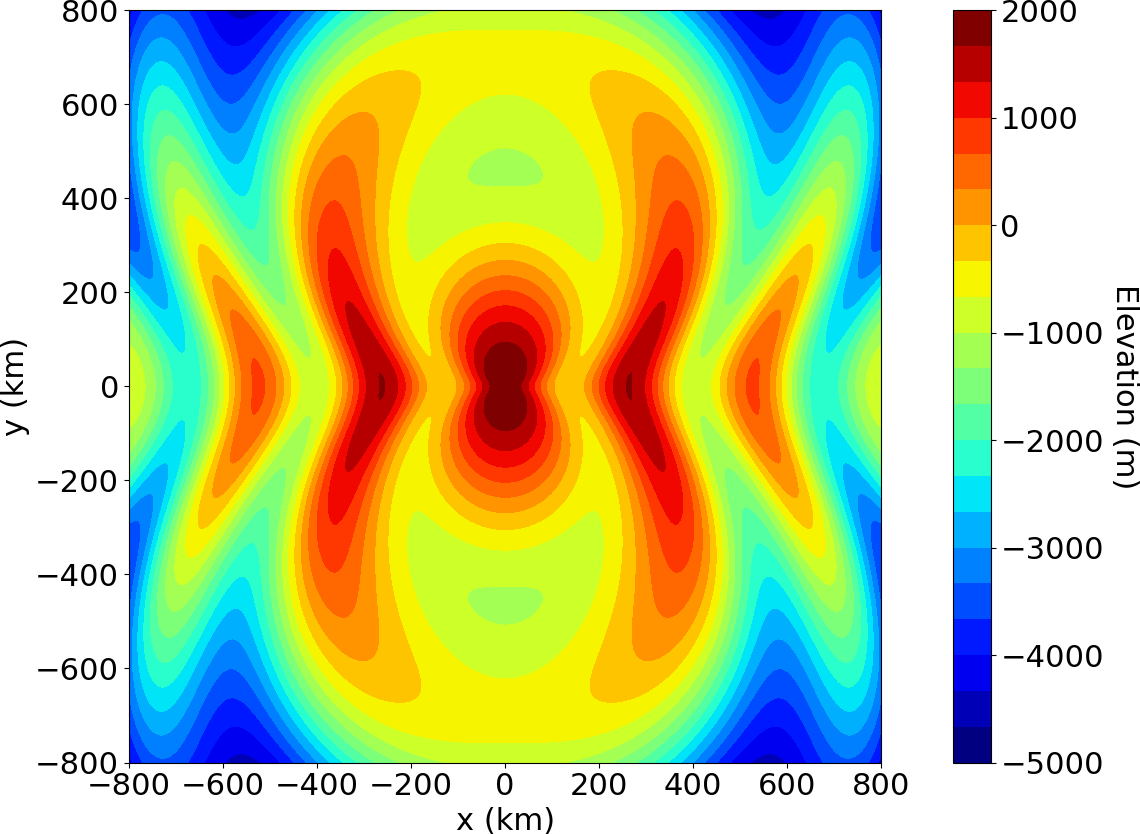
\includegraphics[width=0.45\linewidth]{../fig/Thule_2D}
		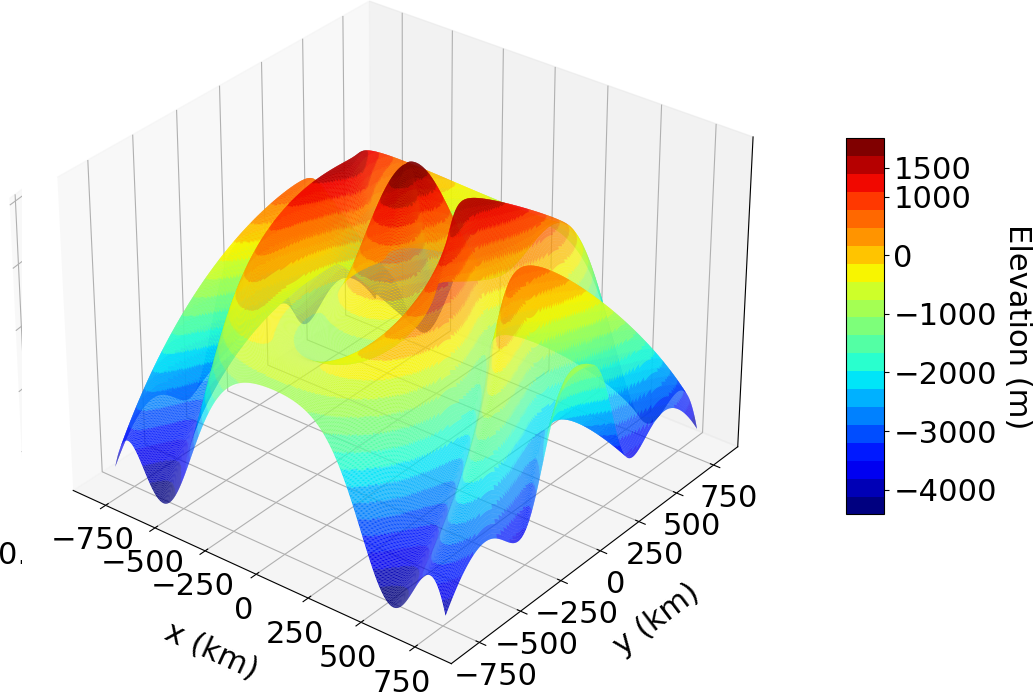
\includegraphics[width=0.45\linewidth]{../fig/Thule_3D}
		\caption{Thule bedrock topography 3D. On the left side the top view, and on the right side a lateral view.}
		\label{Thule_3D}
	\end{figure}
	\begin{figure}[!h]
	\centering
	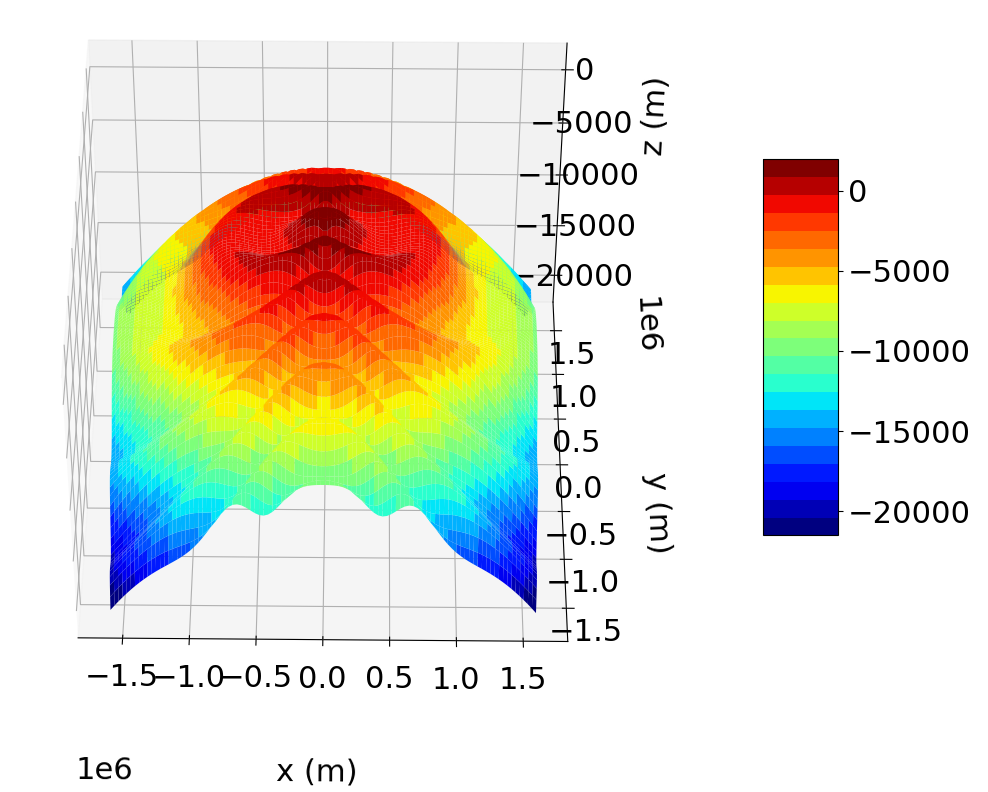
\includegraphics[width=0.45\linewidth]{../fig/Thule_3D1}
	\caption{Thule bedrock topography 3D with a front view.}
	\label{Thule_3D1}
\end{figure}
\subsection{Boundary conditions}
Boundary conditions are needed in order to solve differential equations. It will be assumed that:
\begin{itemize}
	\item The bedrock is impermeable (The vertical component of the ice flow velocity is 0). 
	\item The flow follows the Weertman friction law.
	\item Mass accumulation is a constant parameter.
	\item The simulation will be performed on a quarter of the domain since the geometry of the topography is symmetric, which allows having free slip boundary conditions at the left and downsides of the topography, and open boundary conditions at the right and top sides of the domain. 
\end{itemize}
\subsection{Physical constants}
Table \ref{Physical constants 1}shows the constants parameters that were set up for the experiment by the Calvin MIP project at the beginning of the project. 
\begin{table}[!h]
\begin{center}
\caption{Physical constants 1}
\label{Physical constants 1}
\begin{tabular}{|l|l|l|}
\hline
Variable          & Description                 & Units           \\ \hline
$g=9.81$         & Gravitational acceleration  & $ms^{-2}$         \\ \hline
$a_s=0.3$       & Surface mass balance (SMB)  & $ma^{-1}$         \\ \hline
$a_b=0$             & Basal mass balance (BMB)    & $ma^{-1}$         \\ \hline
$\rho i=917$        & Ice density                 & $kg m^{-3}$       \\ \hline
$\rho w=1030$      & Sea water density           & $kg m^{-3}$       \\ \hline
$A= 2.9377x10^{-9}$ & Ice rate factor             & $KPa^{-3}a^{-1}$  \\ \hline
$n=3$               & Flow law stress exponent    &                 \\ \hline
$C=0.001$           & basal slipperiness          & $ma^{-1}Kpa^{-3}$ \\ \hline
$m=3$               & Sliding law stress exponent &                 \\ \hline
$d2a=365.2422$     & days in a year           & days         \\ \hline
\end{tabular}
\end{center}
\end{table}

After modifications were done in the experiment proposal, the final values used in the simulations are the ones listed in Table \ref{Physical constants}
\begin{table}[!h]
\begin{center}
\caption{Physical constants}
\label{Physical constants}
\begin{tabular}{|l|l|l|}
\hline
Variable          & Description                 & Units           \\ \hline
$g=9.81$         & Gravitational acceleration  & $ms^{-2}$         \\ \hline
$a_s=0.3$       & Surface mass balance (SMB)  & $ma^{-1}$         \\ \hline
$a_b=0$             & Basal mass balance (BMB)    & $ma^{-1}$         \\ \hline
$\rho i=917$        & Ice density                 & $kg m^{-3}$       \\ \hline
$\rho w=1028$      & Sea water density           & $kg m^{-3}$       \\ \hline
$A= 2.9377x10^{-9}$ & Ice rate factor             & $KPa^{-3}a^{-1}$  \\ \hline
$n=3$               & Flow law stress exponent    &                 \\ \hline
$C=0.001$           & basal slipperiness          & $ma^{-1}Kpa^{-3}$ \\ \hline
$m=3$               & Sliding law stress exponent &                 \\ \hline
$s2a=31556926$     & Seconds in a year           & seconds         \\ \hline
\end{tabular}
\end{center}
\end{table}

For the computation of $u_b=2$, we used the Weertman style sliding law:
\begin{equation}
    u_b = C\tau _b^m
\end{equation}
where C is the basal slipperiness and $\tau _b$ is the basal shear stress.
In order to enter these values into the Elmer code, we need to convert all units to Elmer units, namely: MPa, meter, and years. It means that all units that are derivated from time in seconds, must be converted to time in years using the time equivalence proposed in the project and all units or values expressed in terms of KPa must be multiplied by a factor of $10^{-3}$ to be converted to MPa.
Also, to compute the basal sliding velocity $u_b$, Elmer uses the term $\beta$ that is related to $u_b$ by:
\begin{equation}
    \tau = \beta u_b^{\frac{1}{m}}
\end{equation}
So, we have:
\begin{equation}
    u_b = (\frac{\tau}{\beta})^m;
\end{equation}
\begin{equation}
    u_b = \frac{1}{\beta^m} \tau^m
\end{equation}
Using the notation from equation (1), we can say that $C=  \frac{1}{\beta^m}$. So, we can compute $\beta$ as:
\begin{equation}
    \beta=(\frac{1}{C})^{\frac{1}{3}}
\end{equation}
If we replace C by its value given in table \ref{Physical constants}, we get $\beta= 10^4 Pa m^{\frac{-1}{3}} a^{\frac{1}{3}}$ which converted to Mpa will give us a value of 10.

\subsubsection{Numerical parameters}
The numerical resolution will be our variable physical parameter, which we will vary from 10 km, 5 km, 2 km, 1 km, 500 m, and 250 m. 
\subsubsection{External forcing}
We will assume that the only external force acting is gravity ($g=9.81 m/s^2$), which is translated to the weight of the ice sheet and the flotation force of this in the ocean water.
\subsubsection{Initial condition}
The simulation departs from no iced configuration. 
As stated before, the flow will follow the linear Weertman friction law at the base of the ice sheet:
\begin{equation}
	\tau_b=\beta u;
\end{equation}
Where $\tau$ is the friction shear stress, $\beta$ is the basal friction coefficient, and $u$ is the velocity.
Comparisons were made using friction coefficients ranging from $\beta=10^{-8}$ to simulate a friction close to 0, to $\beta=10^{-2}$. This coefficient is also the one chosen to perform the simulations. 
\subsubsection{Time step}
The Courant-Friedrichs-Lewy (CFL) condition is a necessary condition to solve numerical partial differential equations. It states that the distance a variable travels between two-time steps must be smaller than the distance between two points of the mesh \cite[]{courant1967partial}. It is needed that:
\begin{equation}
	C=\frac{u\Delta t}{\Delta x}<Cmax;
\end{equation}
With C the courant number, $u$ the magnitude of the velocity, $\Delta t$ the time step, $\Delta x$ the horizontal resolution, and Cmax = 1. This implies then, for a given mesh:
\begin{equation}
	\Delta t < \frac{\Delta x}{u};
\end{equation}
This is a safe approximation. Cmax then has to be estimated by running different parameters in the simulation and seeing if it converges or not. In order to satisfy the CFL condition, a good starting point is 1 year, since it works properly and converges even for a resolution of 1km.
However, in this experiment, it is asked to report the results every 10 years, and for this reason, we will save the results of the simulation with a frequency of 10 years. 

\section{Results}
As mentioned before, the simulations using Elmer/Ice use unstructured meshes, as shown in the left-hand side of figure \ref{meshes} for a 10km resolution mesh. This is very helpful in terms of simulating complex geometries, for example, the thule configuration.

	\begin{figure}[!h]
		\centering
		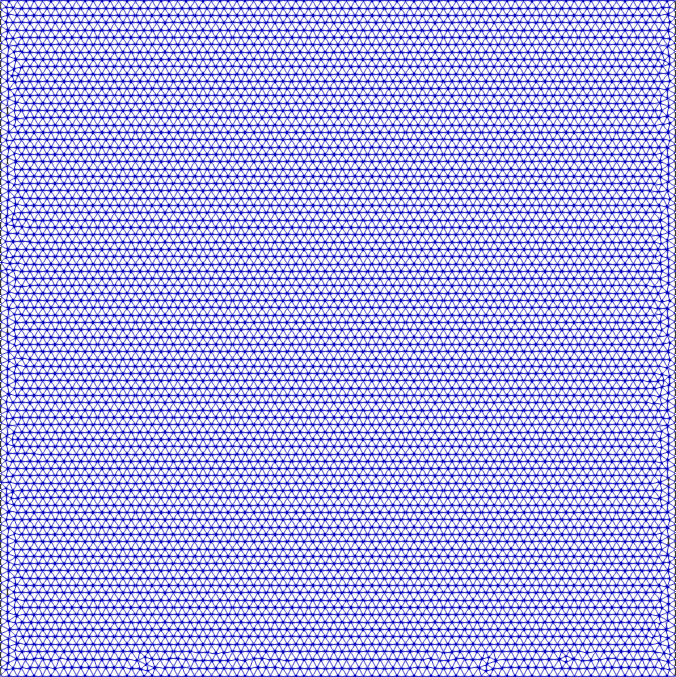
\includegraphics[width=0.45\linewidth]{../fig/non_structured_grid_10km.png}
            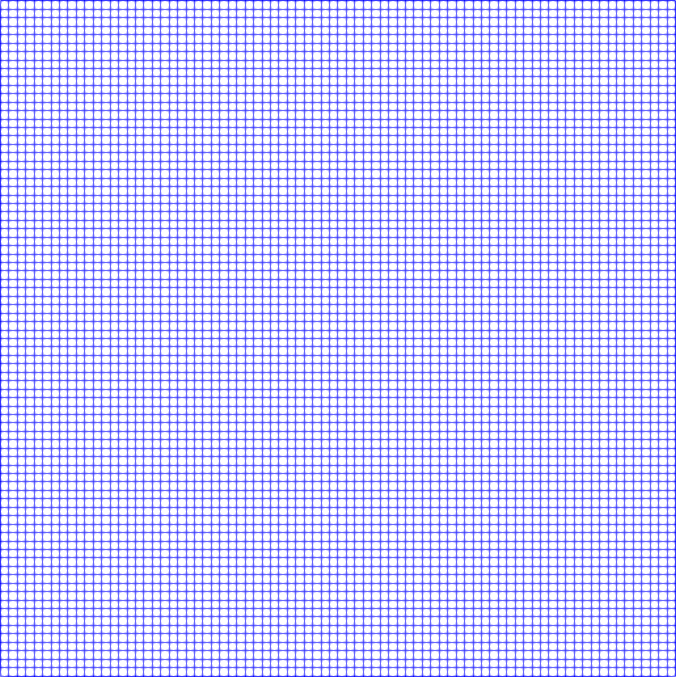
\includegraphics[width=0.45\linewidth]{../fig/regular_grid_10km.png}
		\caption{a) 10km resolution non-structured mesh used in Elmer/Ice. b) Regular structured mesh for 10km resolution.}
		\label{meshes}
	\end{figure}
 
 However, once the simulation is done and to better interpret the results obtained, we need to build a structured mesh, because it is ideal for these time-domain simulations this way we can  easily identify elements and nodes when plotting time-dependent or spacial-dependent graphics. In our case, our objective of interest will be the spacial behavior or dynamic of the glacier since we will analyze the position of the grounding line after the steady state is reached. To build the structured mesh, we performed an interpolation made from the unstructured mesh values of the nodes, namely we interpolate per each node the value of the variables of interest with the values of these variables in the non-structured mesh. This way we know which position the node is in, and we can plot figures spacial-dependent, namely, we can plot the value of different variables, for example, the velocity components, as a function of the horizontal position. 
 
\subsection{Cone configuration}

For this first experiment proposed, the simulations were run varying the resolution from 10km and up to 1km. In figure \ref{figCONO1} we show a qualitative representation of the simulation results for the different resolutions, where we also run 50 and 20km resolution just to have a better idea of how this change in the resolution has an impact in the results. In these figures, the blue part represents the grounded part of the domain, and the grey part represent the floating part. This way we can identify the changes in the transition from grounded to not grounded, namely the grounding zone. We can see also how, as we go closer to a minimum resolution, the differences start to be not that notorious. 

\begin{figure}[!h]
	\centering % <-- added
	\begin{subfigure}{0.25\textwidth}
		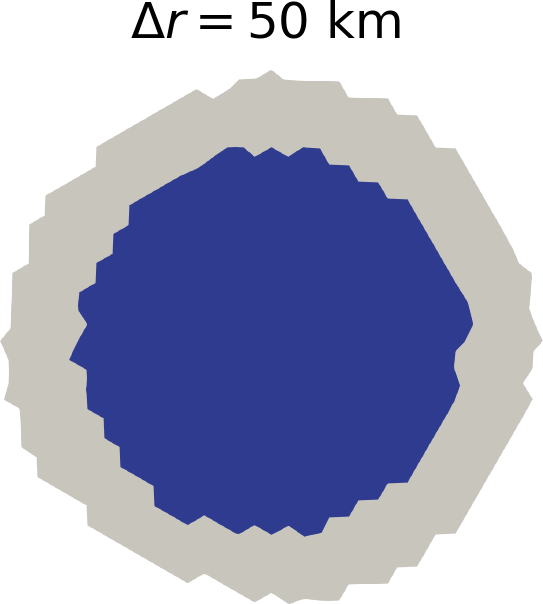
\includegraphics[width=\linewidth]{../fig/Grounded_zone_50km_CONE.png}
		\caption{Grounded zone (blue) and floating ice (grey) for 50km resolution}
		\label{figCONE50KM}
	\end{subfigure}\hfil % <-- added
	\begin{subfigure}{0.25\textwidth}
		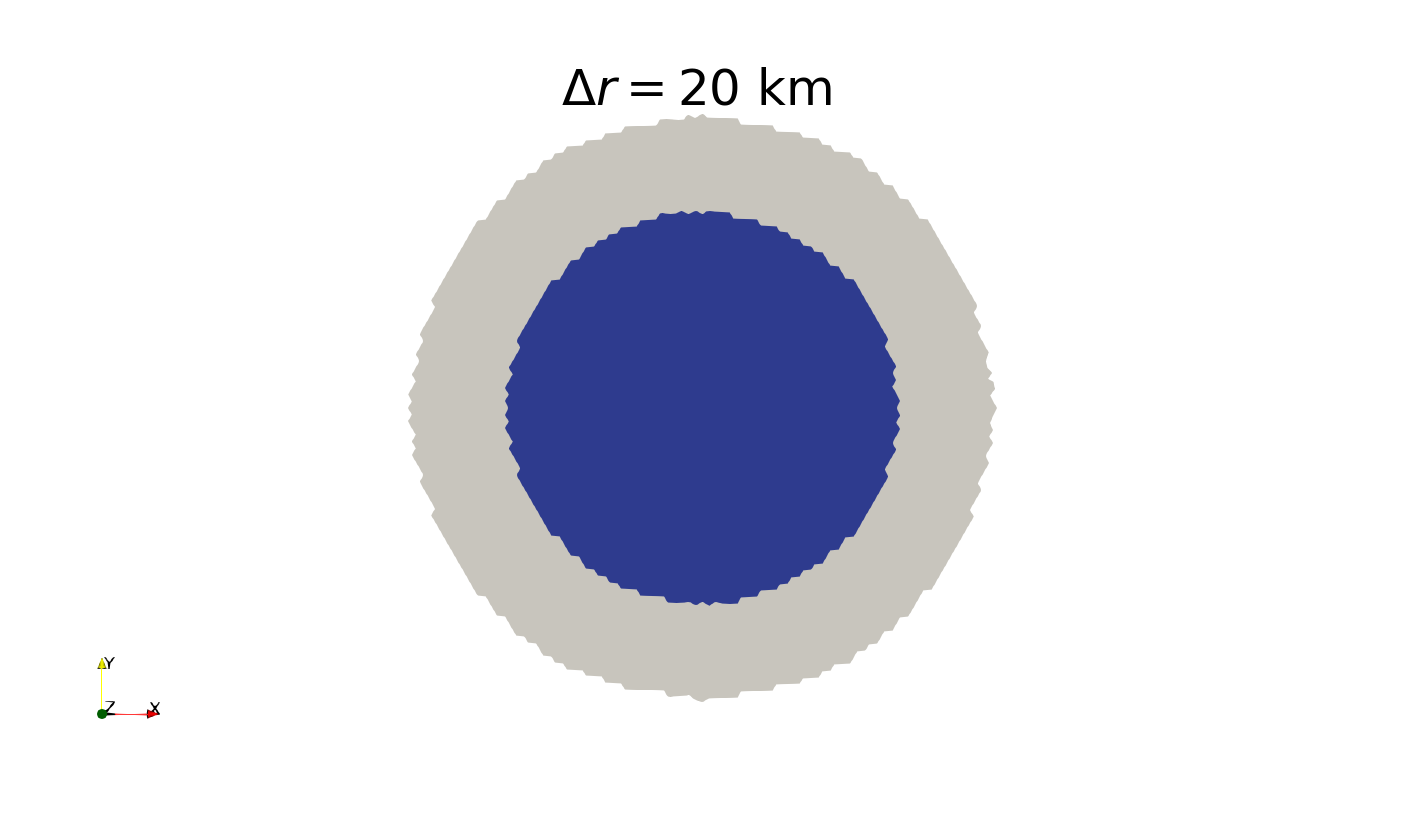
\includegraphics[width=\linewidth]{../fig/Grounded_zone_20km_CONE.png}
		\caption{Grounded zone (blue) and floating ice (grey) for 20km resolution}
		\label{figCONE20}
	\end{subfigure}\hfil % <-- added
	\begin{subfigure}{0.25\textwidth}
		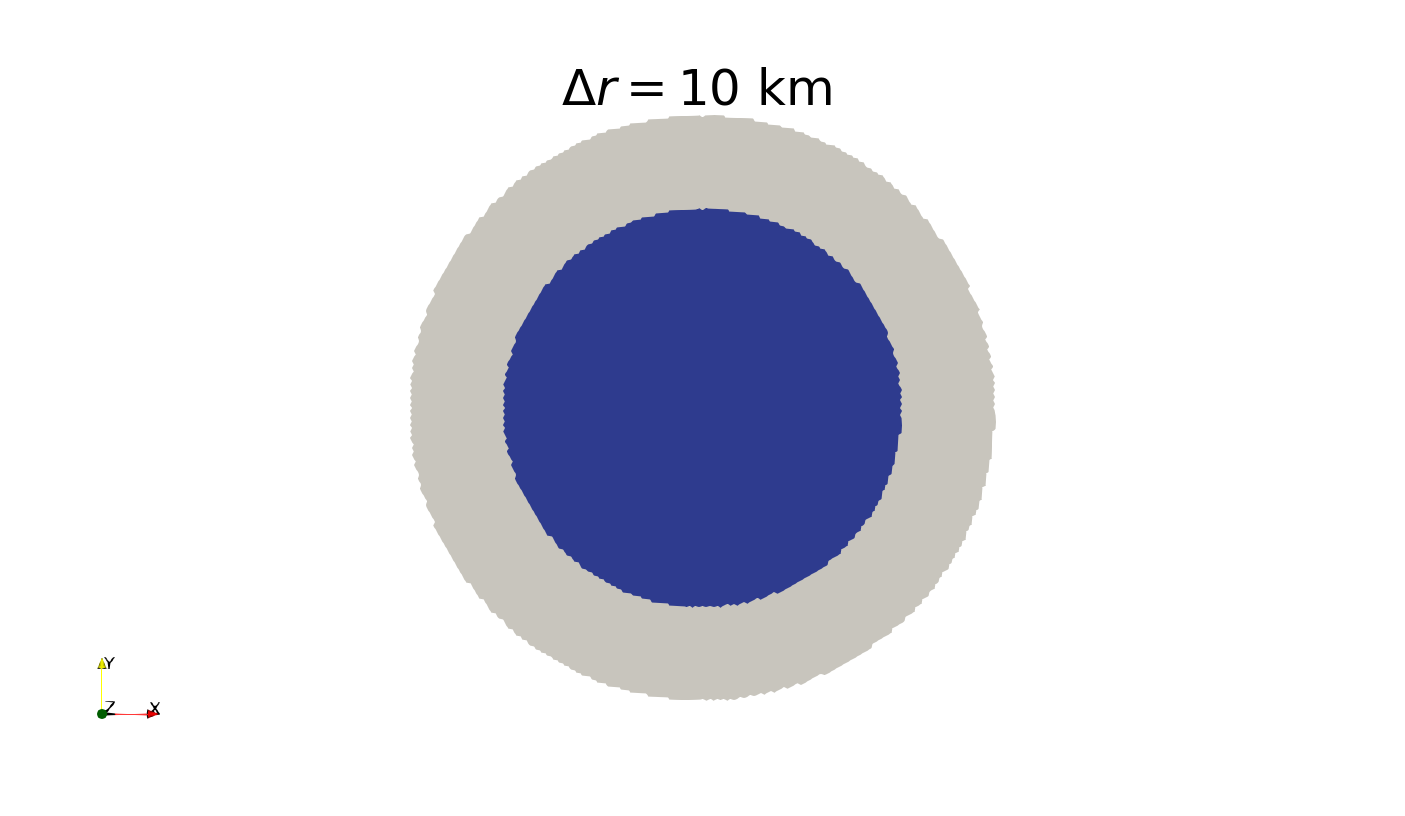
\includegraphics[width=\linewidth]{../fig/Grounded_zone_10km_CONE.png}
		\caption{Grounded zone (blue) and floating ice (grey) for 10km resolution}
		\label{figCONE10KM}
	\end{subfigure}
	
	\medskip
	\begin{subfigure}{0.25\textwidth}
		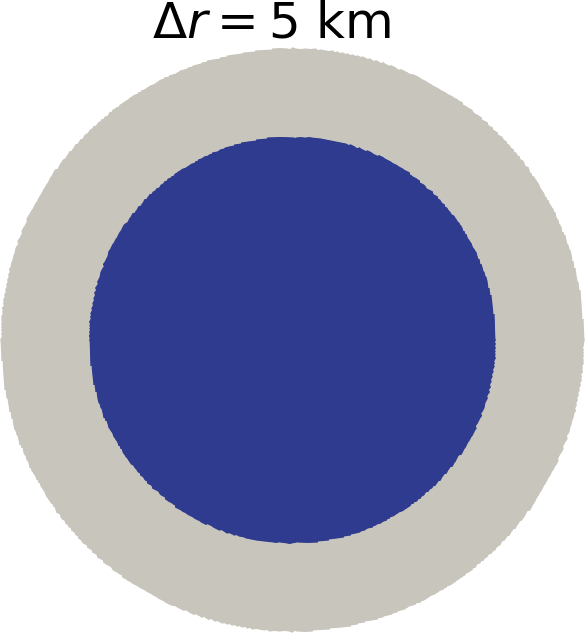
\includegraphics[width=\linewidth]{../fig/Grounded_zone_5km_CONE.png}
		\caption{Grounded zone (blue) and floating ice (grey) for 5km resolution}
		\label{figCONE5}
	\end{subfigure}\hfil % <-- added
	\begin{subfigure}{0.25\textwidth}
		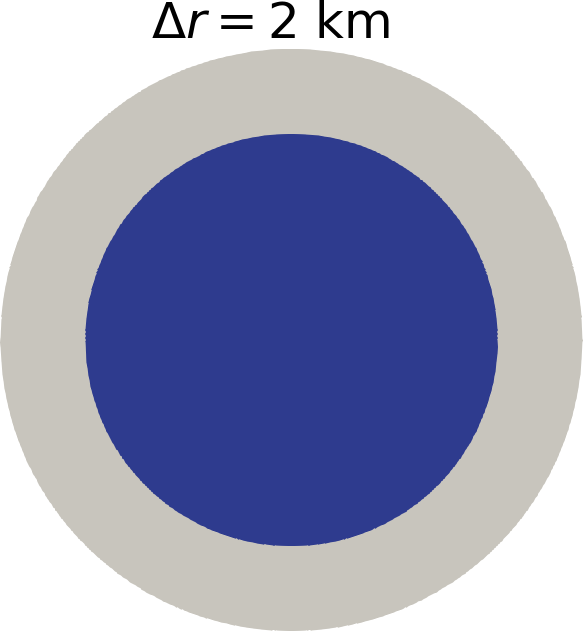
\includegraphics[width=\linewidth]{../fig/Grounded_zone_2km_CONE.png}
		\caption{Grounded zone (blue) and floating ice (grey) for 2km resolution}
		\label{figCONE2}
	\end{subfigure}\hfil % <-- added
	\begin{subfigure}{0.25\textwidth}
		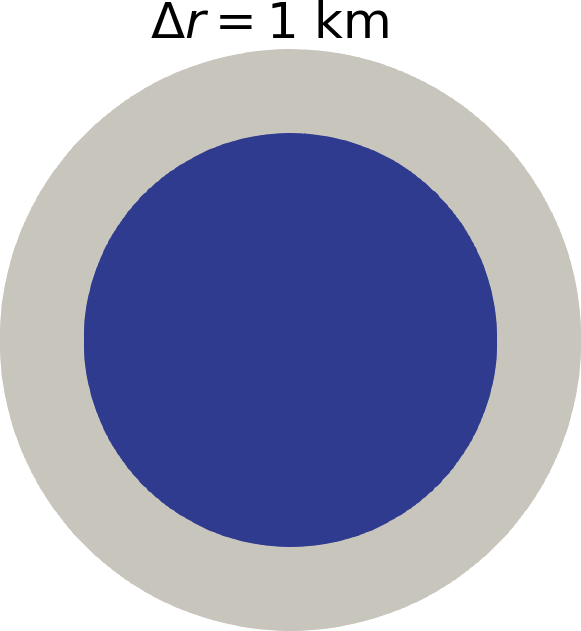
\includegraphics[width=\linewidth]{../fig/Grounded_zone_1km_CONE.png}
		\caption{Grounded zone (blue) and floating ice (grey) for 1km resolution}
		\label{CONE1KM}
	\end{subfigure}
	\caption{Impact of the resolution in the grounded area for the cone circular domain.}
	\label{figCONO1}
\end{figure}

In figure \ref{Cone_scheme}, we see an schematic representation of the results for the cone circular domain experiment. For the analysis of these results, the ice thickness of the profile was analysed along 8 linear profiles, namely A,B,C,D,E,F,G and H for the domain complete, as shown in figure \ref{Schematic_Cone}, and in figure \ref{Profiles_cone} we see all the positions and the ice thickness along the different profiles in the same figure. The point or zone where the lower part of the ice sheet stops being in contact with the bedrock is the grounding line. In this figure it is also highlighted the quarter of the domain in figure \ref{Schematic_Cone} and its three profiles A,B,C since, as mentioned before, both simulations for the domain complete and the quarter domain were run to compare the results.

\begin{figure}
	\centering
	\begin{subfigure}{.5\textwidth}
		\centering
		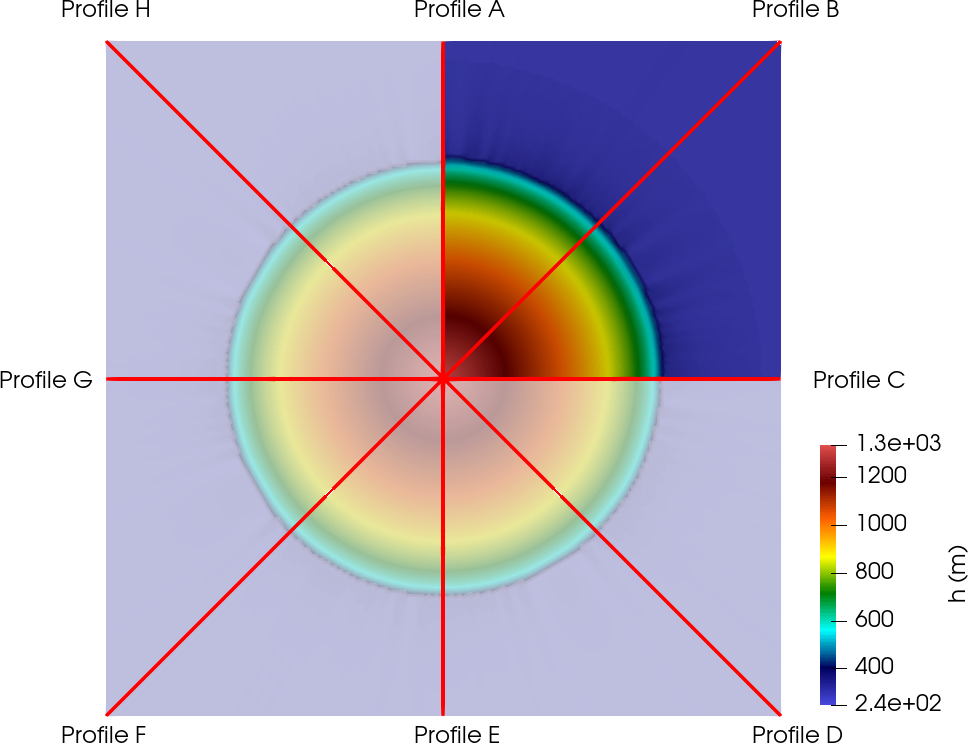
\includegraphics[width=0.99\linewidth]{../fig/Profiles_Cone_combined_domains.png}
		\caption{Profiles for Cone circular domain}
		\label{Schematic_Cone}
	\end{subfigure}%
	\begin{subfigure}{.5\textwidth}
		\centering
		\includegraphics[width=0.99\linewidth]{../fig/Profiles_Cone_domain_sin_fondo.png}
		\caption{Ice thickess per profile}
		\label{Profiles_cone}
	\end{subfigure}
	\caption{Schematic representation of the circular domain ice sheet showing the ice thickness results along the profiles proposed.}
	\label{Cone_scheme}
\end{figure}

To have a better idea of the simulations convergence, in figure \ref{h_and_h_velocities_cone} it is shown on the left sides all the values of ice thickness in meters per each resolution, and on the left sides the values of the ice thickness velocity obtained, namely the rate of change of the ice thickness in meters per year. The range of these values, maximum and minimum per resolution are very low (less than 0,001 m/y), which is a brief image that shows that the simulations reached a steady state with a low estimation error. 

Once both results were obtained, for the domain complete and the quarter domain, the next step consists in quantify the grounding line position per each resolution along the profiles proposed. For this, a function that can be denominated grounding line was created, and this function was defined as the product of the bedrock position and a grounding mask. This grounded mask is a step function created, which a value of -1 is assigned to the grounded ice, and 1 to the part of the ice that is no longer in contact with the bedrock, namely:

\[ \begin{cases} 
	-1 & bedrock = z_b \\
	1 & z_b \leq bedrock   
\end{cases}
\]

Using this mask, we created the grounding line function as the negative product of this mask and the bedrock (the negative sign is only implemented for convention). From the fact that this grounding line function is an increasing function, it must have an unique maximum, namely, the point where the function changes sign. This maximum means the point where $z_b$ is no longer equal to bedrock position, so starting from this point, the lower part of the ice sheet is not grounded any more. This maximum value of the grounding line function corresponds, physically, to the point where the grounding line or zone is along an x-profile. Knowing this point, the distance from the origin of our coordinate system to that point can be computed, knowing the x and y coordinates of this point, as the norm if this vector, this distance determines the grounding line position, in meters, along an x axis. The results were calculated in two parts: along three profiles A,B and C for the quarter of the domain, and along all the profiles from A to H for the domain complete. For both cases, per each resolution the mean, maximum and minimum value of the grounding line position was calculated. 

\begin{figure}[!h]
	\centering % <-- added
	\begin{minipage}[t]{.25\textwidth}
		\begin{subfigure}{\textwidth}
			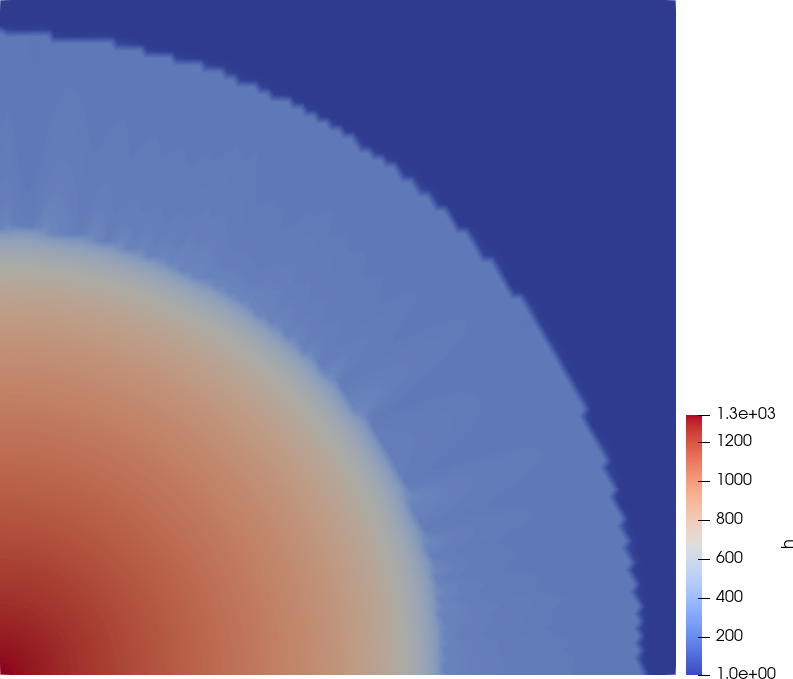
\includegraphics[width=\linewidth]{../fig/h_10km_quarter.png}
			\caption{Ice thickness for 10km resolution.}
			\label{h10km}
		\end{subfigure}\hfil % <-- added
		\begin{subfigure}{\textwidth}
			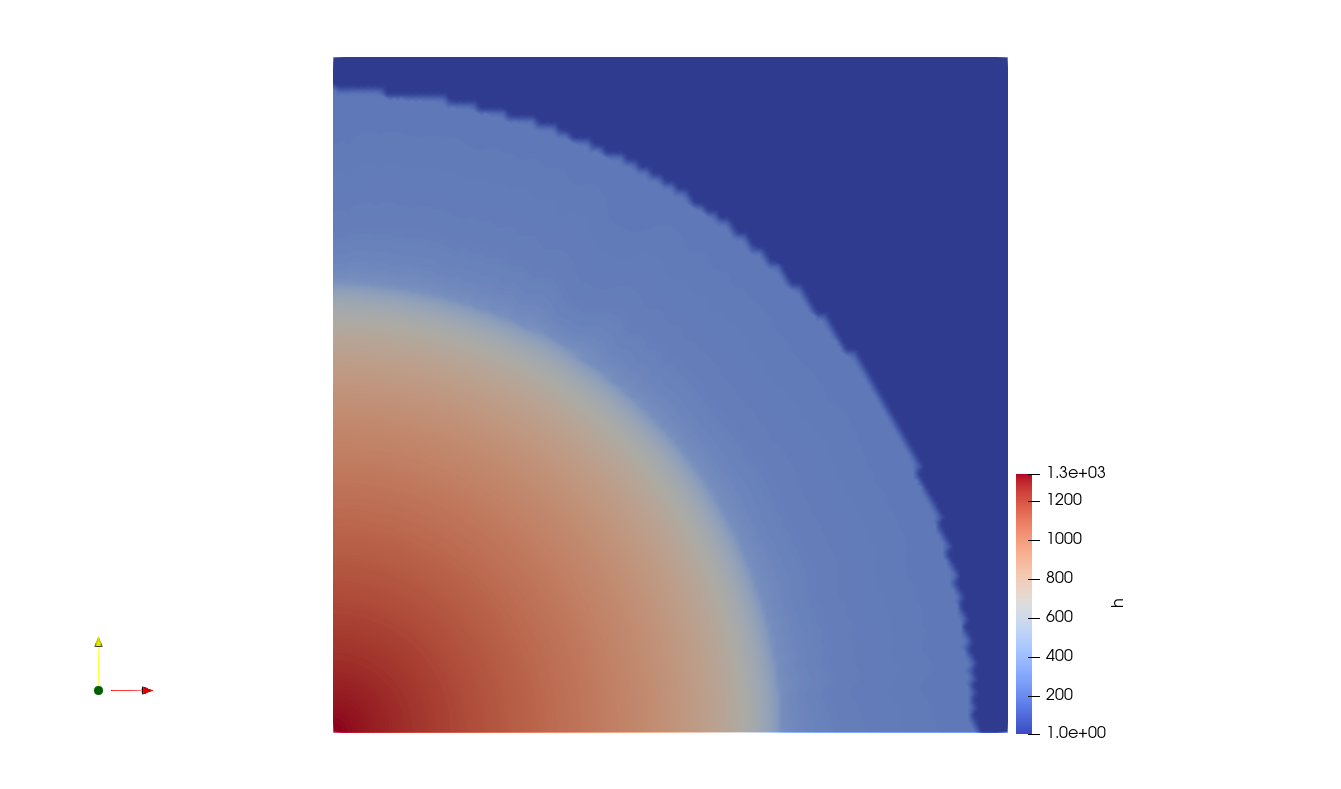
\includegraphics[width=\linewidth]{../fig/h_5km_quarter.png}
			\caption{Ice thickness 5km resolution.}
			\label{h5km}
		\end{subfigure}\hfil % <-- added
		\begin{subfigure}{\textwidth}
			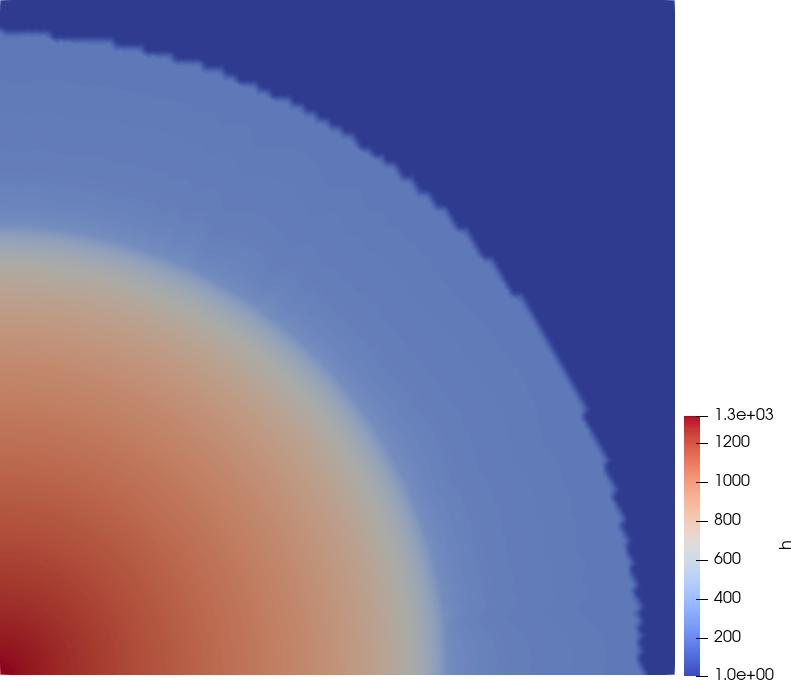
\includegraphics[width=\linewidth]{../fig/h_2km_quarter.png}
			\caption{Ice thickness for 2km resolution.}
			\label{h2km}
		\end{subfigure}
		\begin{subfigure}{\textwidth}
		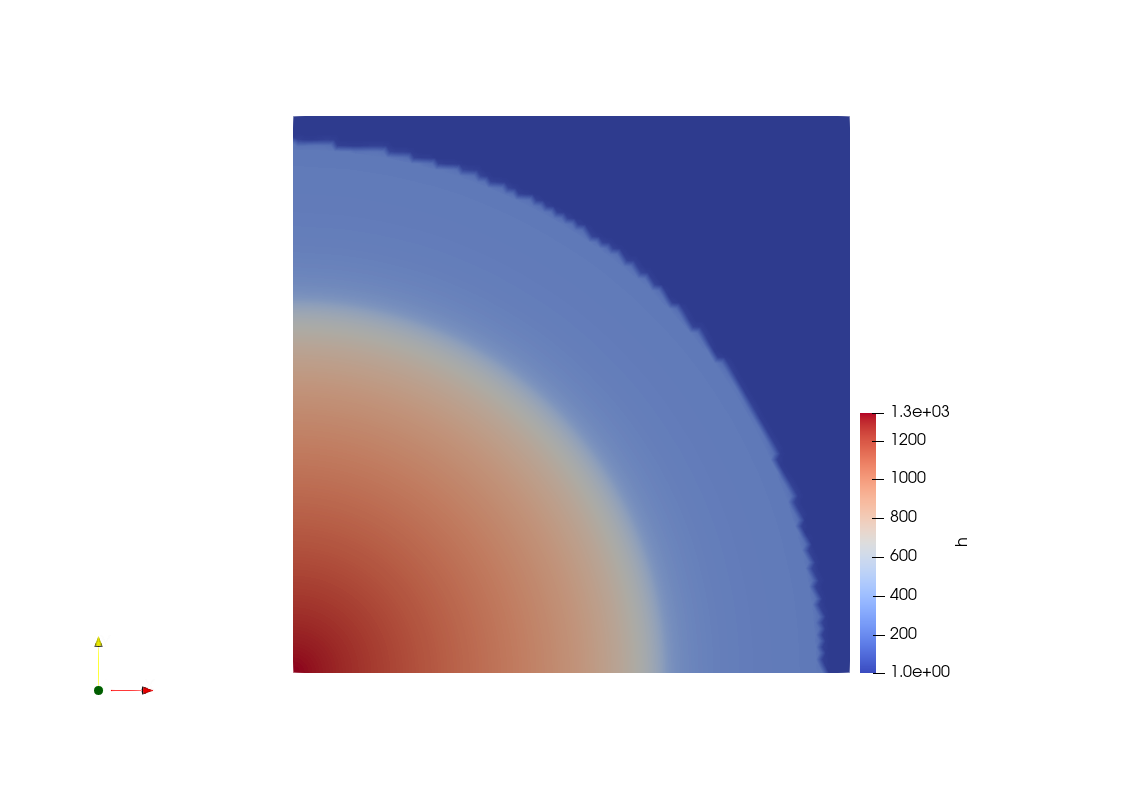
\includegraphics[width=\linewidth]{../fig/h_1km_quarter.png}
		\caption{Ice thickness for 1km resolution.}
		\label{h1km}
	    \end{subfigure}
	\end{minipage}\hfil
	\begin{minipage}[t]{.25\textwidth}
		\begin{subfigure}{\textwidth}
			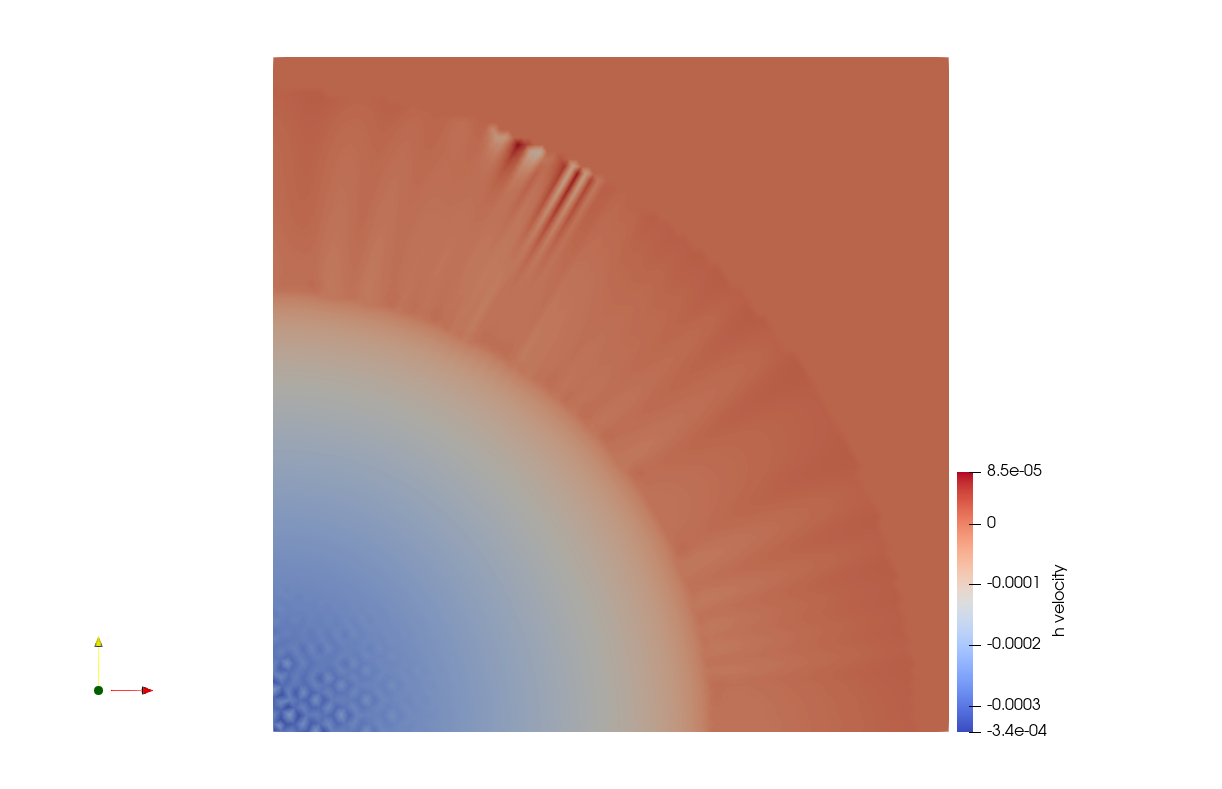
\includegraphics[width=\linewidth]{../fig/hvelocity_10km_quarter.png}
			\caption{Ice sheet thickness velocity 10km.}
			\label{hvelocity10km}
		\end{subfigure}\hfil % <-- added
		\begin{subfigure}{\textwidth}
			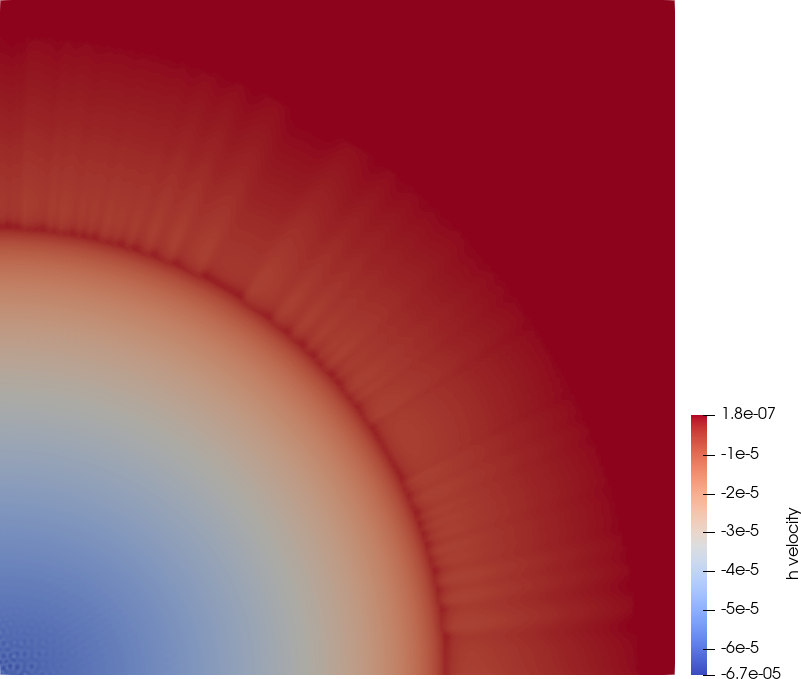
\includegraphics[width=\linewidth]{../fig/hvelocity_5km_quarter.png}
			\caption{Ice sheet thickness velocity 5km}
			\label{hvelocity5km}
		\end{subfigure}\hfil % <-- added
		\begin{subfigure}{\textwidth}
			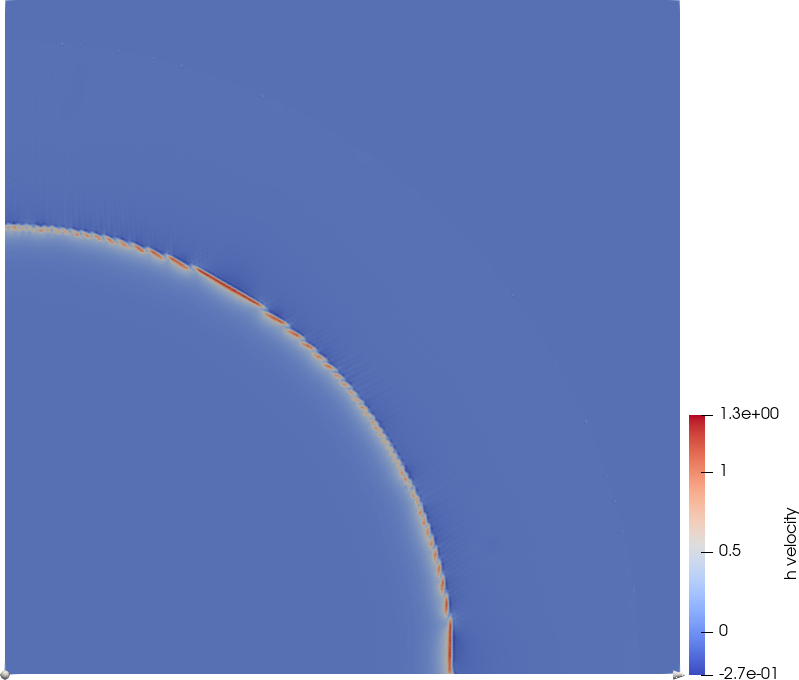
\includegraphics[width=\linewidth]{../fig/hvelocity_2km_quarter.png}
			\caption{Ice sheet thickness velocity 2km}
			\label{hvelocity2km}
		\end{subfigure}
				\begin{subfigure}{\textwidth}
			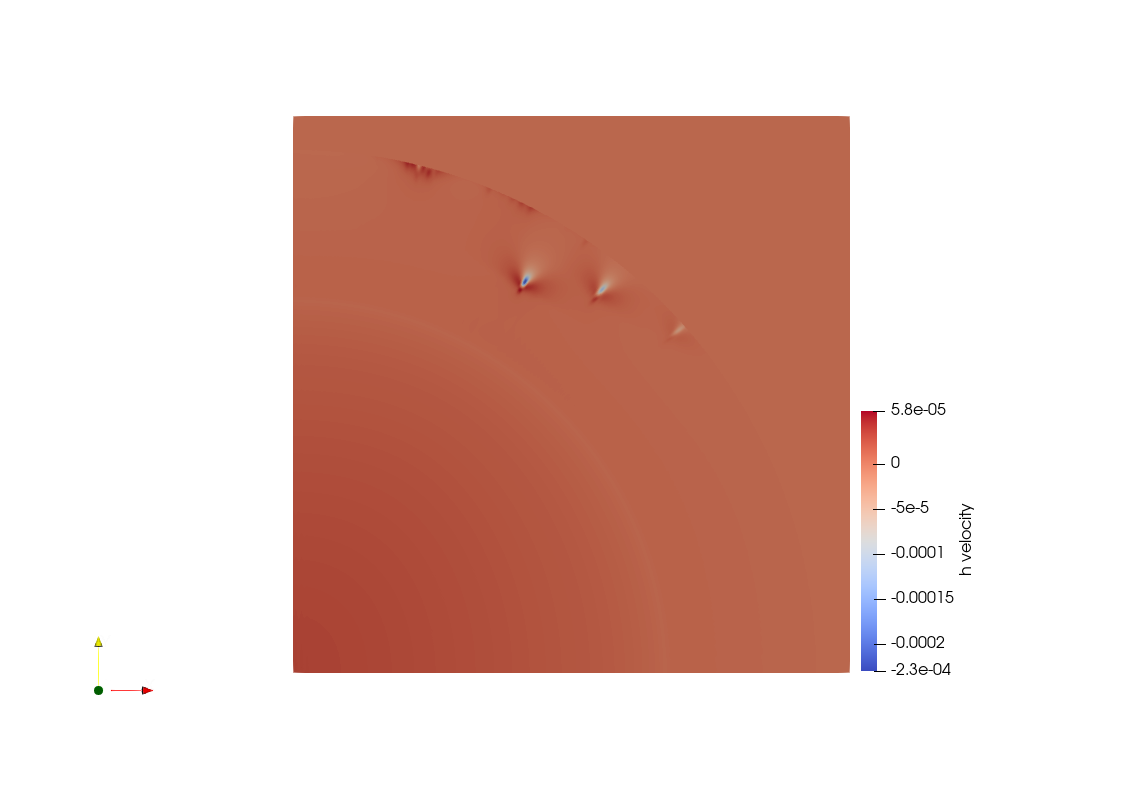
\includegraphics[width=\linewidth]{../fig/hvelocity_1km_quarter.png}
			\caption{Ice sheet thickness velocity 1km}
			\label{hvelocity1km}
		\end{subfigure}	
	\end{minipage}
	\caption{Ice thickness and ice sheet thickness rate of change for quarter domain per each resolution after steady state.}
	\label{h_and_h_velocities_cone}
\end{figure}

These mean, maximum and minimum value of the grounding line position per resolution is shown in figure \ref{Grounding_lines__CONE_comparison} for both case studies, the quarter and complete domain. In the y-axis we have the grounding line position in meters, that is the distance calculated from an origin to the grounding line or zone computed before using the function. This distance is computed as the norm of a vector (x,y) that defines this grounding line position. 

\begin{figure}[!h]
	\centering
	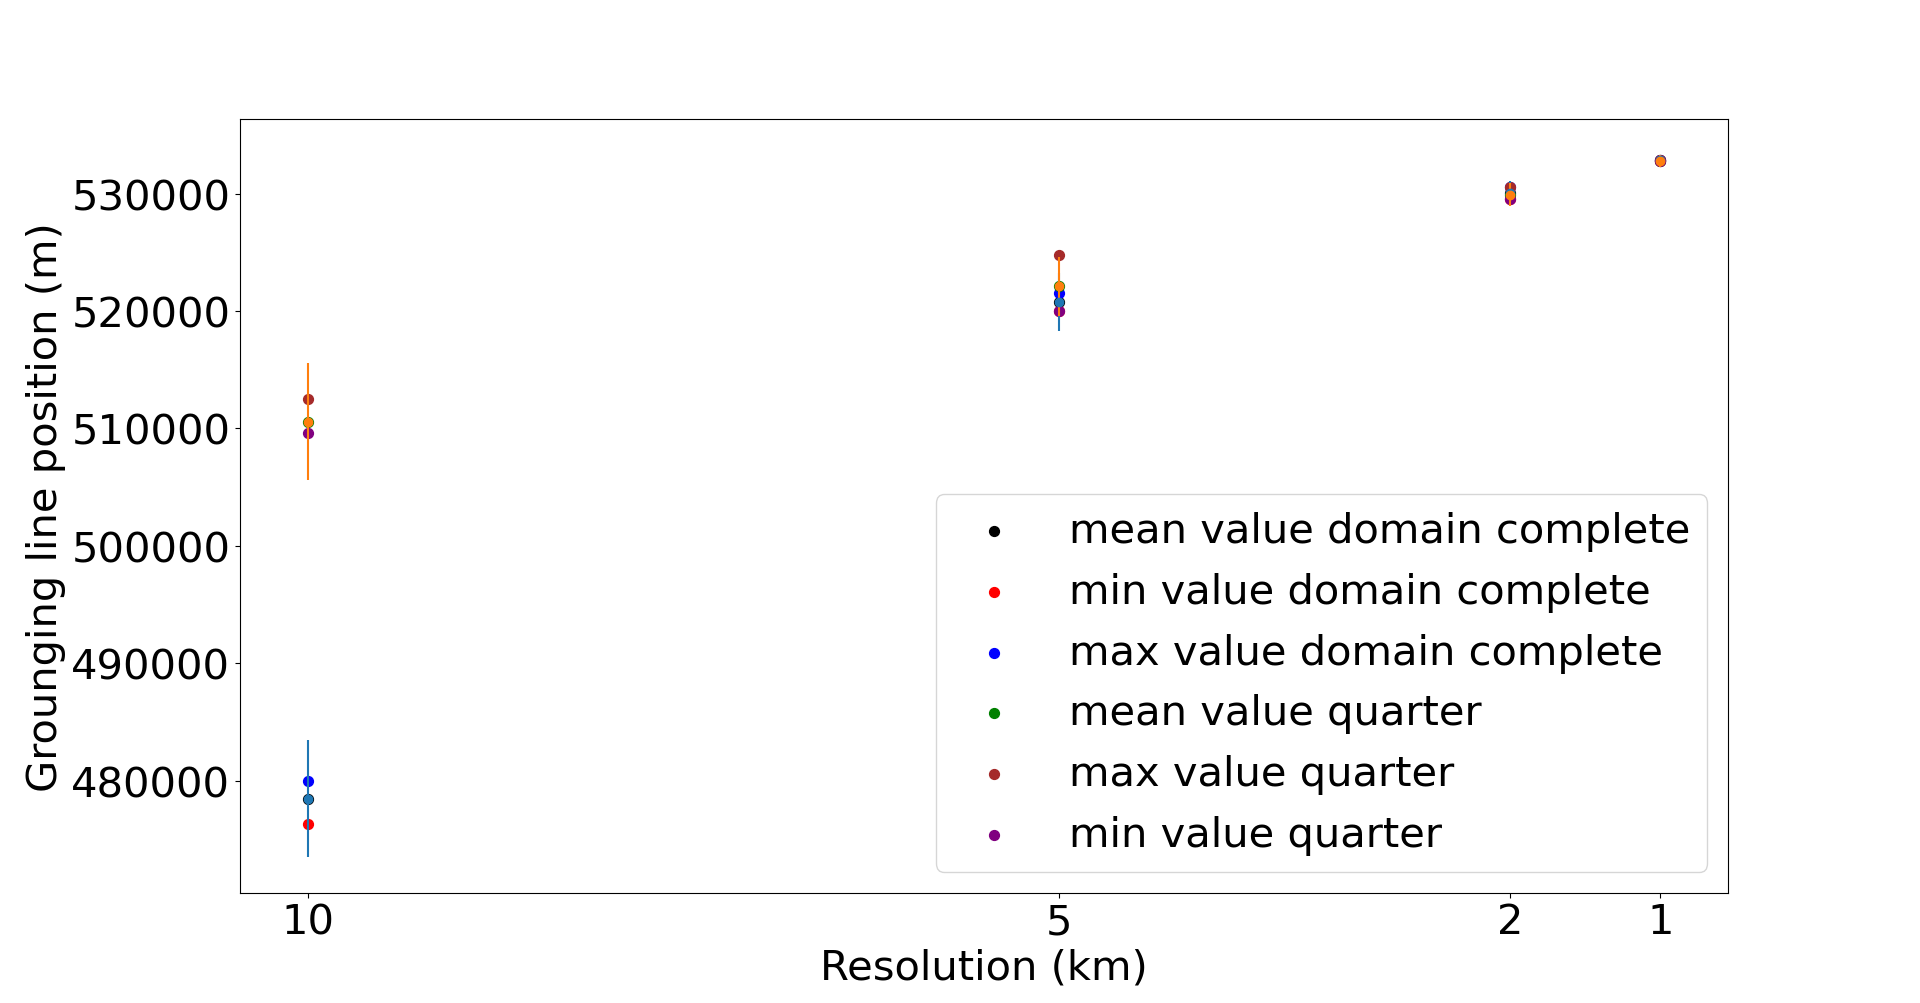
\includegraphics[width=0.8\linewidth]{../fig/Figure_CONE_GL_positions.png}
	\caption{Grounding line positions as a function of the resolution for quarter and complete circular cone domain.}
	\label{Grounding_lines__CONE_comparison}
\end{figure}

For both cases, the complete and quarter of the domain results, it is associated an error bar for the mean values of the grounding line position. The yellow bar corresponds to the quarter domain mean value error bar, and the blue bar corresponds to the complete domain mean value error bar. The error associated was determined as half of the value for each resolution (5km for the 10km resolution, 2.5km for 5km, 1km for 2km and 500m for 1km resolution).

It can be observed how, for greater resolutions as 10km, the results have a difference of around 20km for the grounding line position between the quarter of the domain and the complete domain results, but for lower resolutions these difference starts to be lower. 

\subsection{Thule configuration}
For the second part of the experiments, the results for the thule configuration were obtained for a quarter of the domain and the domain complete, and following the Calving MIP inter comparison project, the simulations using this topography were run using 10,5,2 and 2 km meshes. The figure \ref{Thule_profiles_capronas_and_halbranes} shows the schematic representation of the thule domain experiment results. Similar to the Cone domain experiment, here it is proposed to analyse the results along profiles called Caprona and Halbrane. The figure \ref{Profiles_Thule} highlights the quarter of the domain, since the simulations were also run for this part of the domain to compare it with the complete system. In this case the results were analysed for Caprona profiles and separately for the Halbrane profiles. In figures \ref{Capronas_thule} and \ref{Halbranes_thule} it can be observed the ice thickness along each one of the profiles and so the position of the grounding line.

\begin{figure}[!h]
  \begin{subfigure}[c]{.52\linewidth}
    \centering
    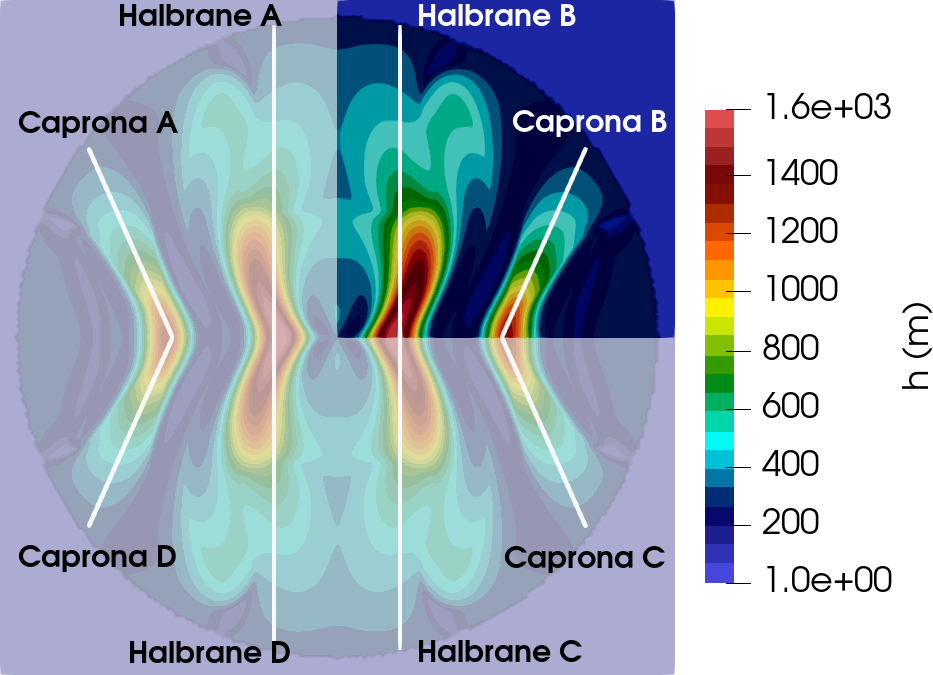
\includegraphics[width=\linewidth]{../fig/Profiles_Thule_combined_domains_2_con_fondo.png}%
    \caption
      {%
        Profiles for the thule domain%
        \label{Profiles_Thule}%
      }%
  \end{subfigure}\hfill
  \begin{tabular}[c]{@{}c@{}}
    \begin{subfigure}[c]{.48\linewidth}
      \centering
      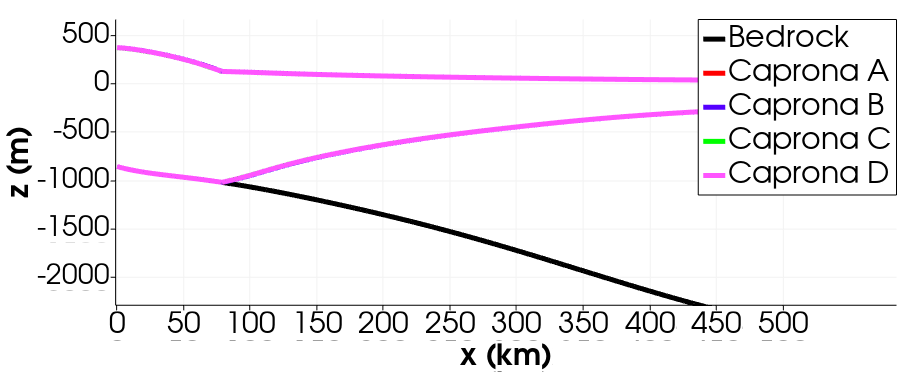
\includegraphics[width=\linewidth]{../fig/Capronas_Thule_Domain_con_fondo.png}%
      \caption
        {%
          Ice thickness along each Caprona profile%
          \label{Capronas_thule}%
        }%
    \end{subfigure}\\
    \noalign{\bigskip}%
    \begin{subfigure}[c]{.48\linewidth}
      \centering
      \includegraphics[width=\linewidth,page=2]{../fig/Halbranes_thule_domain_con_fondo.png}%
      \caption
        {%
          Ice thickness along each Halbrane profile%
          \label{Halbranes_thule}%
        }%
    \end{subfigure}
  \end{tabular}
  \caption
    {%
      Schematic representation of thule ice sheet showing ice thickness along Caprona and Halbrane profiles.%
      \label{Thule_profiles_capronas_and_halbranes}%
    }
\end{figure}

In figure \ref{Thule_resolutions} a qualitative representation of the simulations results can be observed as well to have a visualization of the impact of the resolution on the grounded area of the domain. Similar to the results for the Cone circular domain, the blue part represents the grounded part and the grey part represents the part of the ice that is floating in water. 

\begin{figure}[!h]
	\centering % <-- added
	\begin{subfigure}{0.25\textwidth}
		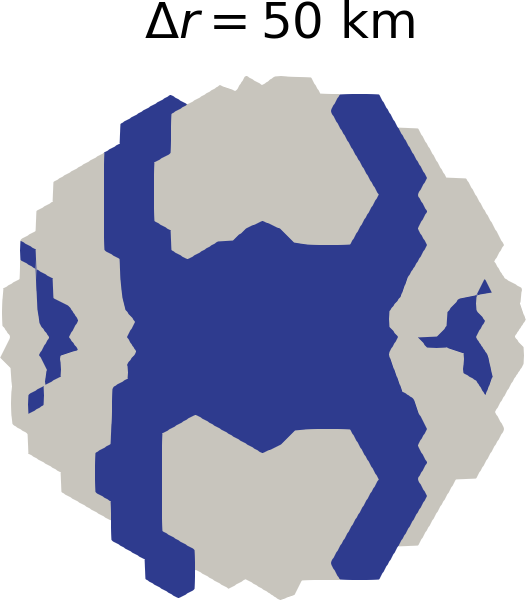
\includegraphics[width=\linewidth]{../fig/Grounded_zone_50km.png}
		\caption{image1}
		\label{fig:1}
	\end{subfigure}\hfil % <-- added
	\begin{subfigure}{0.25\textwidth}
		\includegraphics[width=\linewidth]{../fig/Grounded_zone_20km.png}
		\caption{image2}
		\label{fig:2}
	\end{subfigure}\hfil % <-- added
	\begin{subfigure}{0.25\textwidth}
		\includegraphics[width=\linewidth]{../fig/Grounded_zone_10km.png}
		\caption{image3}
		\label{fig:3}
	\end{subfigure}
	
	\medskip
	\begin{subfigure}{0.25\textwidth}
		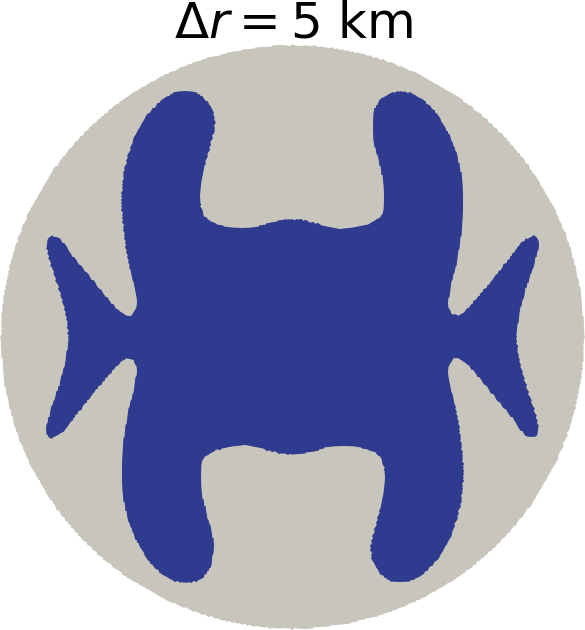
\includegraphics[width=\linewidth]{../fig/Grounded_zone_5km.png}
		\caption{image4}
		\label{fig:4}
	\end{subfigure}\hfil % <-- added
	\begin{subfigure}{0.25\textwidth}
		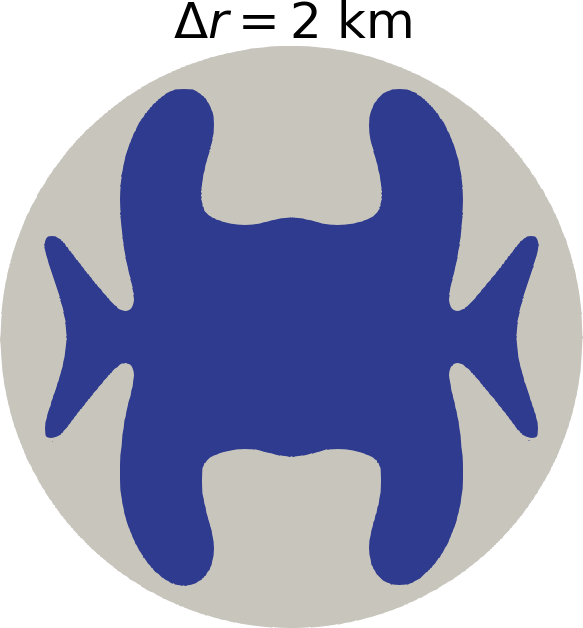
\includegraphics[width=\linewidth]{../fig/Grounded_zone_2km.png}
		\caption{image5}
		\label{fig:5}
	\end{subfigure}\hfil % <-- added
	\begin{subfigure}{0.25\textwidth}
		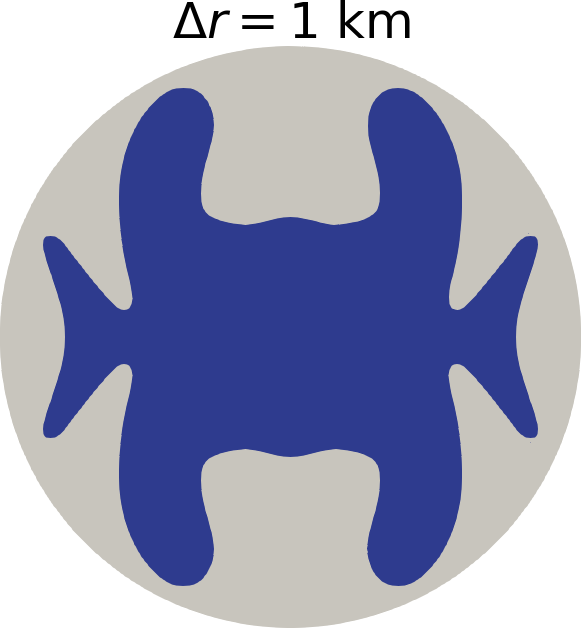
\includegraphics[width=\linewidth]{../fig/Grounded_zone_1km.png}
		\caption{image6}
		\label{fig:6}
	\end{subfigure}
	\caption{Impact of the resolution in the grounded area}
	\label{Thule_resolutions}
\end{figure}


\subsection{Comparison of parameters for each resolution for the different configurations}
In this part of the experiment, we compared the time spent during the simulations as a function of the number of nodes. The figure \ref{TimeVsNumberofnodes} shows this relation for both experiment, the cirular and the thule profile domain, both for the domain complete. 
The time shown in figure \ref{TimeVsNumberofnodes} is the time spent by the computer using the 32 processors to run the simulations.

	\begin{figure}[!h]
	\centering
	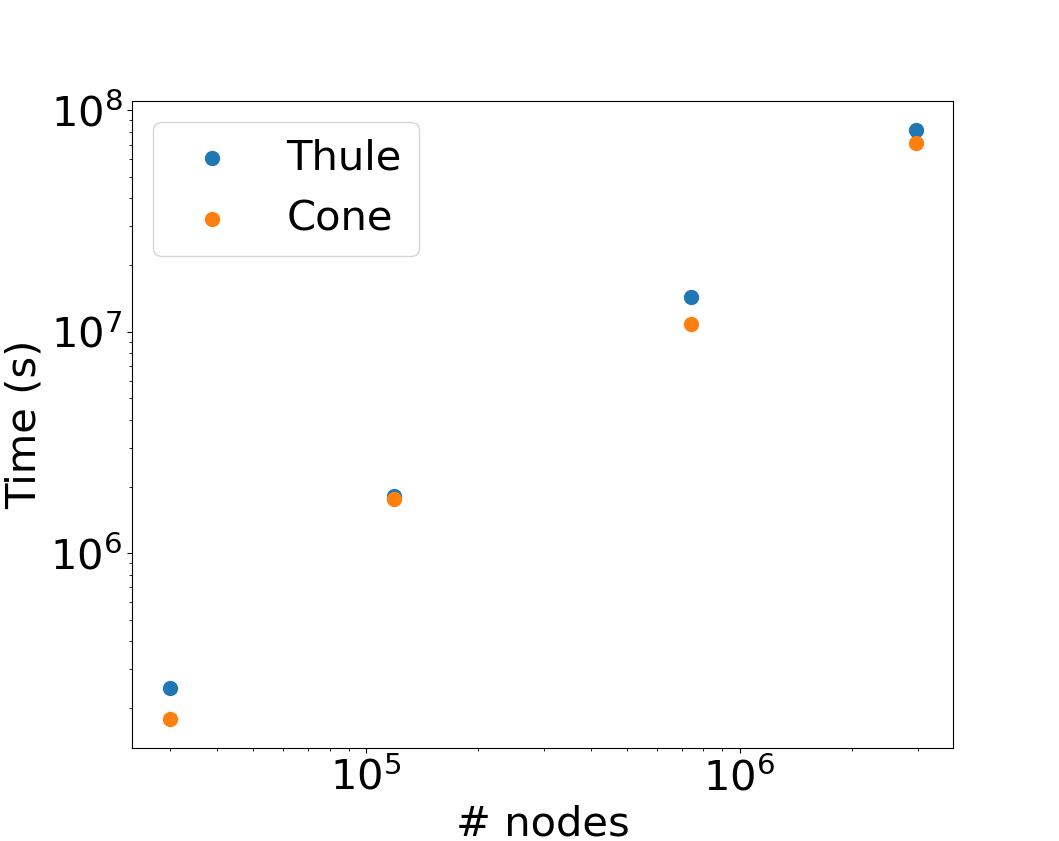
\includegraphics[width=0.9\linewidth]{../fig/TimeVsNumberOfNodes.png}
	\caption{Comparison of the time spent by the simulation as a function of the number of nodes for both configurations.}
	\label{TimeVsNumberofnodes}
	\end{figure}

	\begin{figure}[!h]
	\centering
	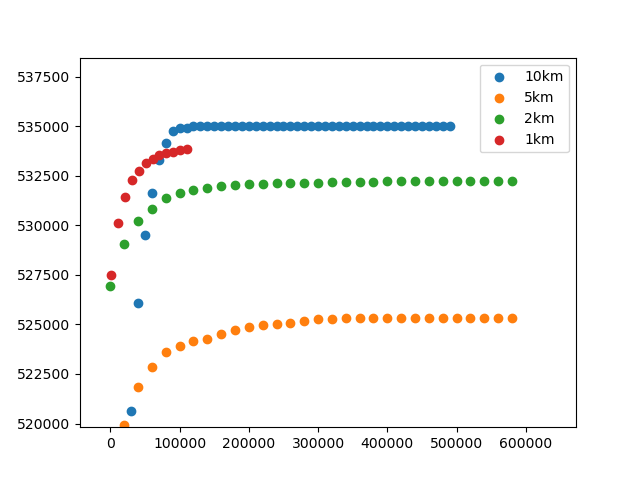
\includegraphics[width=0.9\linewidth]{../fig/Grounding_line_integrated_full_domain_CONE_time.png}
	\caption{Grounding line position as a function of time for different resolutions for the complete circular domain.}
	\label{TimeVsGroundingLinePosition_full}
	\end{figure}


	\begin{figure}[!h]
	\centering
	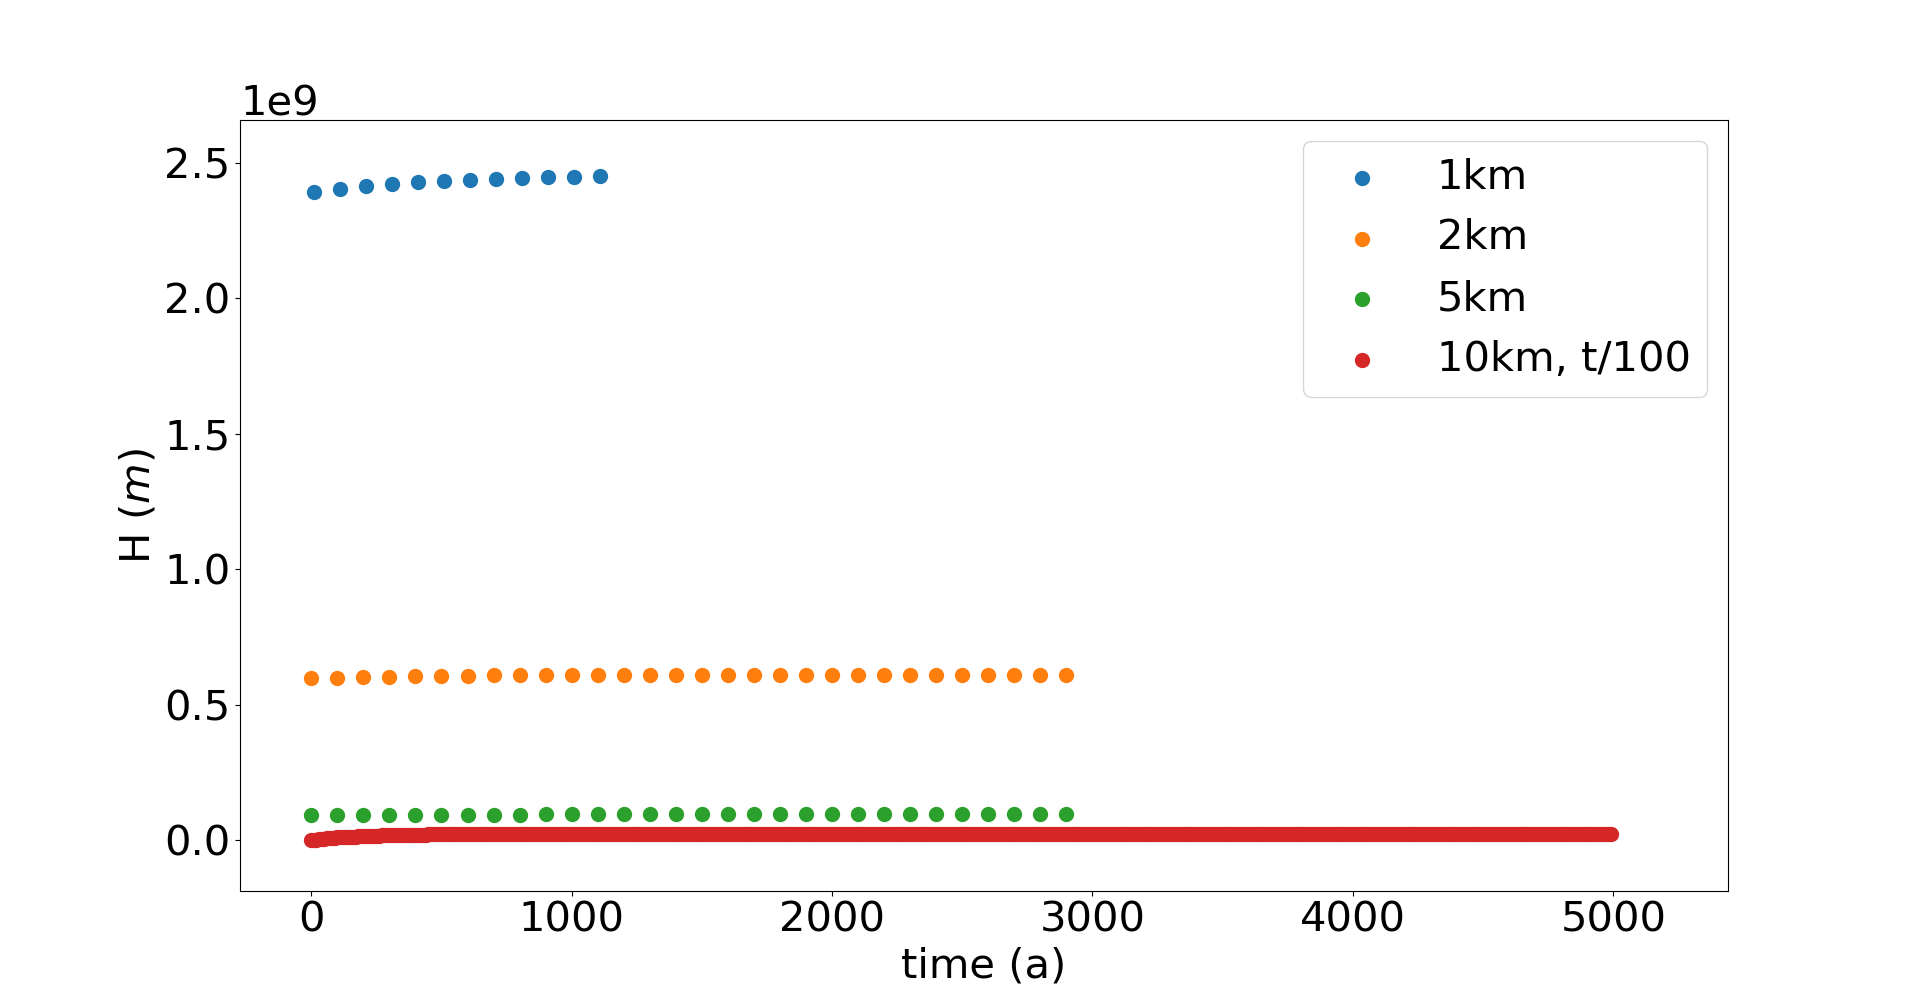
\includegraphics[width=0.45\linewidth]{../fig/H_CONE_full_all_res_vs_time.png}
	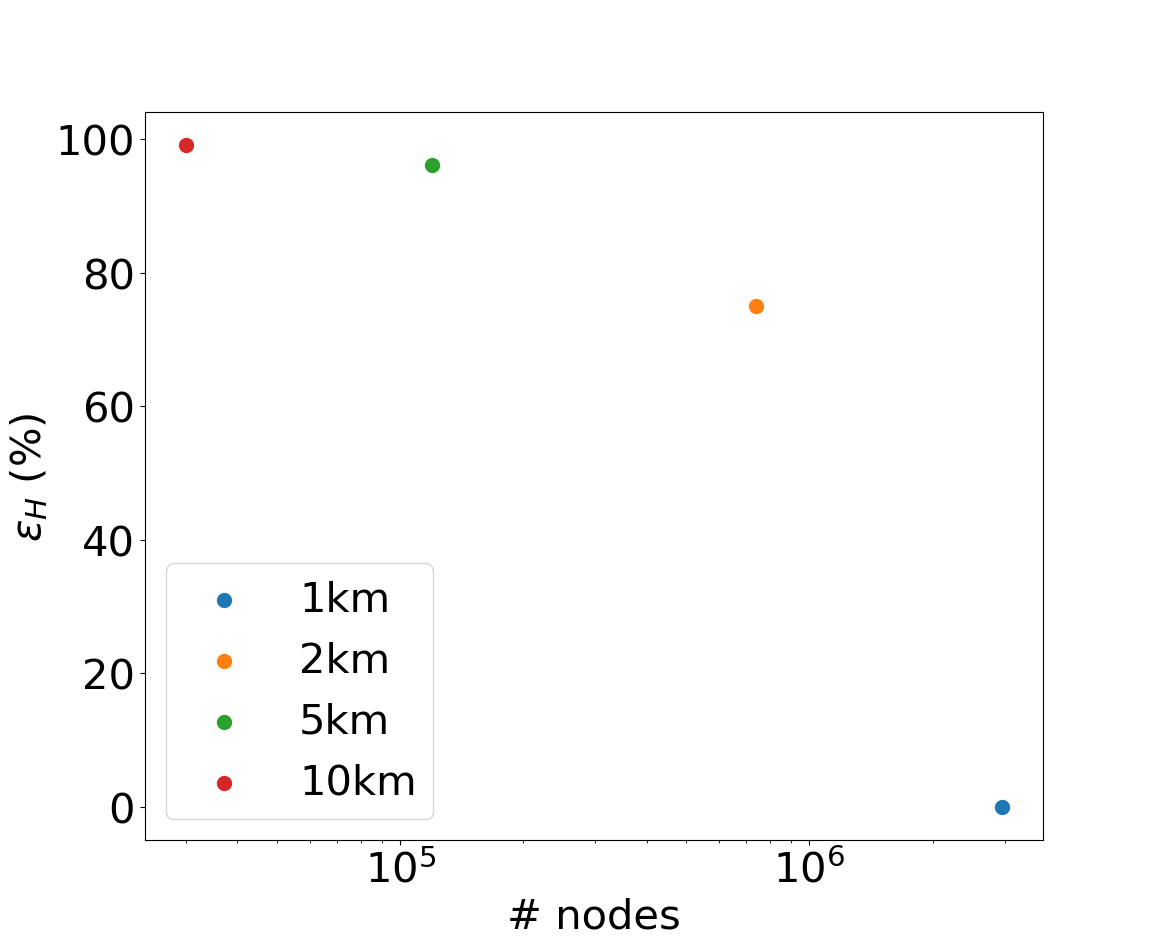
\includegraphics[width=0.45\linewidth]{../fig/H_CONE_full_all_res_vs_num_nodes.png}
	\caption{a) Ice thickness as a function of time. b) Ice thickness as a function of the number of nodes.}
	\label{H_CONE_all_res}
	\end{figure}

	\begin{figure}[!h]
	\centering
	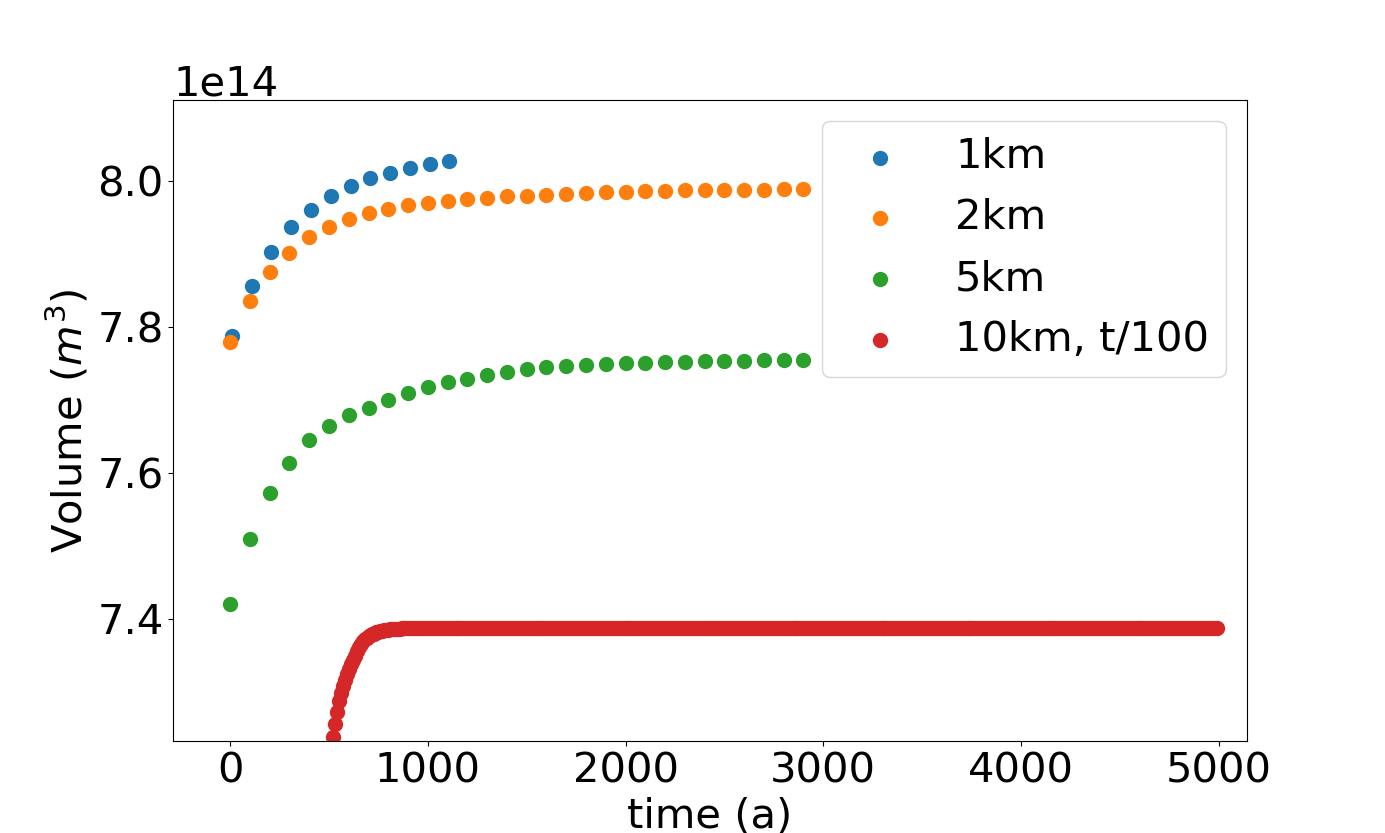
\includegraphics[width=0.45\linewidth]{../fig/Volume_CONE_full_all_res_vs_time.png}
	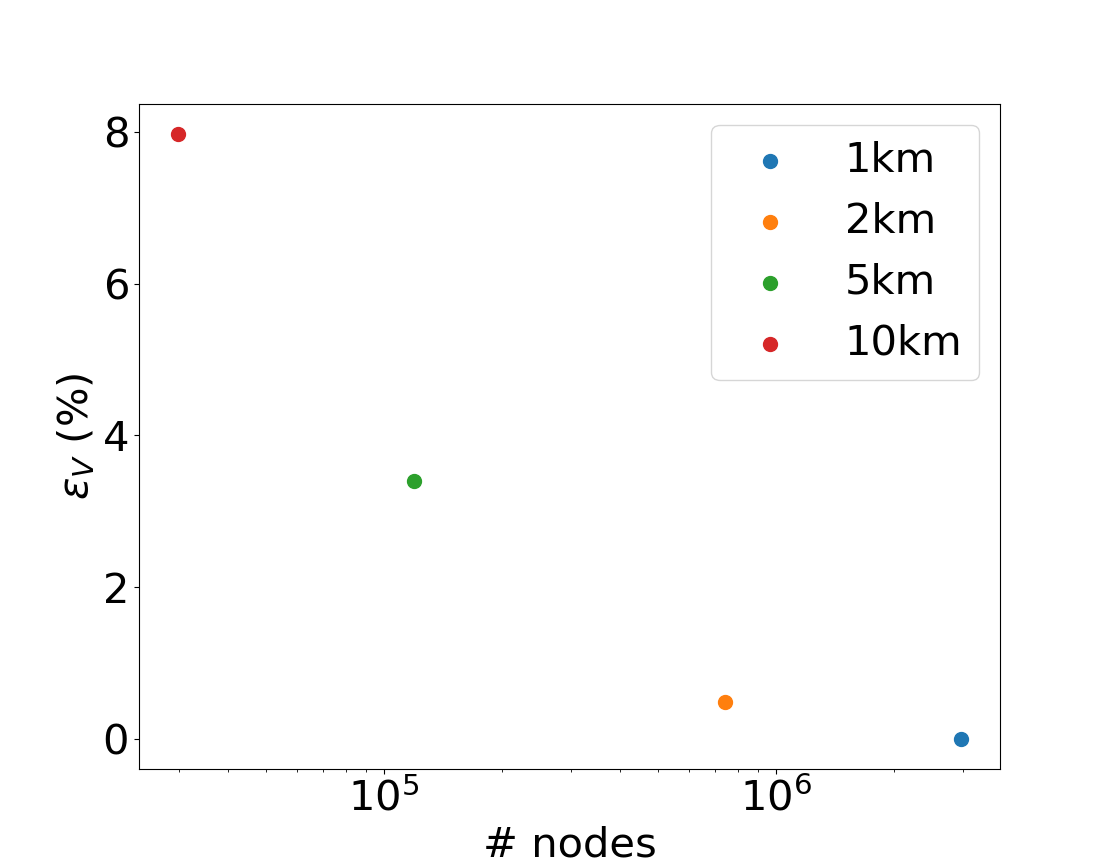
\includegraphics[width=0.45\linewidth]{../fig/Volume_CONE_full_all_res_vs_num_nodes.png}
	\caption{a) Ice volume as a function of time. b) Ice volume as a function of the number of nodes.}
	\label{Volume_CONE_all_res}
\end{figure}


\section{Discussion}
Here we will discuss the differences found between the results obtained for the different spacial resolutions for thule and cone, for the complete domain using the previous constant parameters, and the results obtained for the quarter domain using the new parameters. We will discuss the accuracy of the model for the different resolutions in predicting the position of the grounding line for both types of configurations. We will compare the position of the grounding line as a function of the resolution. 
Also, we will discuss the time spent in the simulations as a function of the number of processors used (plot) and we can try to discuss an optimum number of processors that can be used (will be reviewed).
\section{Conclusion}
We will present our main conclusions of the project. The main objectives that were accomplished and future changes or improvements to do for further research.
   \pagebreak

    \bibliographystyle{apalike}
    \bibliography{./biblio}
\end{document}


